%%%%%%%%%%%%%%%%%%%%%%%%%%%%%%%%%%%%%%%%%%%%%%%%%%%%%%%%%%%%%%%%%%%%%%%%%%%%%%%%%%%%%%%%%%%%%%%%%%%%%%%%%%%%%%%%%%%%%%%%%%%%%
% IV ENCONTRO BRASILEIRO DE MENSURAÇÃO FLORESTAL
%%%%%%%%%%%%%%%%%%%%%%%%%%%%%%%%%%%%%%%%%%%%%%%%%%%%%%%%%%%%%%%%%%%%%%%%%%%%%%%%%%%%%%%%%%%%%%%%%%%%%%%%%%%%%%%%%%%%%%%%%%%%%

%%%%%%%%%%%%%%%%%%%%%%%%%%%%%%%%%%%%%%%%%%%%%%%%%%%%%%%%%%%%%%%%%%%%%%%%%%%%%%%%%%%%%%%%%%%%%%%%%%%%%%%%%%%%%%%%%%%%%%%%%%%%%
% CONFIGURAÇÕES GLOBAIS
%%%%%%%%%%%%%%%%%%%%%%%%%%%%%%%%%%%%%%%%%%%%%%%%%%%%%%%%%%%%%%%%%%%%%%%%%%%%%%%%%%%%%%%%%%%%%%%%%%%%%%%%%%%%%%%%%%%%%%%%%%%%%
\documentclass[12pt,ignorenonframetext,aspectratio=1610]{beamer}
%\documentclass[12pt,ignorenonframetext,aspectratio=1610,compress]{beamer}

\mode<presentation> {
  \usetheme[compress]{Berlin}
  \setbeamercovered{transparent}
  \setbeamertemplate{page number in head/foot}[framenumber]
  %\usecolortheme{default}
  \usefonttheme{structurebold}
  %\useoutertheme{infolines}
  %\definecolor{darkcyan1}{rgb}{0.0, 0.45, 0.45}
  %\definecolor{darkcyan2}{rgb}{0.0, 0.55, 0.55}
  %\definecolor{darkcyan3}{rgb}{0.0, 0.65, 0.65}
  %\definecolor{ivory}{rgb}{1.0, 1.0, 0.94}
  %\definecolor{lightyellow}{rgb}{1.0, 1.0, 0.88}
  %\definecolor{green(pigment)}{rgb}{0.0, 0.65, 0.31}
  %\definecolor{darkseagreen}{rgb}{0.56, 0.74, 0.56}
  %\definecolor{dollarbill}{rgb}{0.52, 0.73, 0.4}
  %\definecolor{emerald}{rgb}{0.31, 0.78, 0.47}
  \definecolor{honeydew}{rgb}{0.94, 1.0, 0.94}
  \definecolor{green(munsell)}{rgb}{0.0, 0.66, 0.47}
  \definecolor{mygreen1}{rgb}{0.0, 0.5, 0.0}
  \definecolor{mygreen2}{rgb}{0.0, 0.5.5, 0.0}
  \definecolor{mygreen3}{rgb}{0.0, 0.6, 0.0}
  \definecolor{mygreen4}{rgb}{0.0, 0.4, 0.0}
  \definecolor{blond}{rgb}{0.98, 0.94, 0.75}
  %%%%%%%%%%%%%%%%%%%%%%%%%%%%%%%%%%%%%%%%%%%%%%%%%%%
  %\definecolor{forestgreen(web)}{rgb}{0.13, 0.55, 0.13}
  %\setbeamercolor{titlelike}{parent=structure,bg=yellow!85!orange} %default wolverine
  
  \setbeamercolor{structure}{fg=black}
  \setbeamercolor{titlelike}{parent=structure,bg=mygreen2,fg=white} %cor caixa e letra do titulo 
  \setbeamercolor{navigation symbols}{fg=green!90, bg=mygreen4}
  %\setbeamercolor{palette sidebar secondary}{fg=yellow,bg=blue}
  %\setbeamercolor{section in sidebar shaded}{fg=black,bg=white}
  %\setbeamercolor{subsection in sidebar shaded}{fg=gray,bg=white}
  \setbeamercolor{frametitle}{bg=mygreen4,fg=honeydew}
  \setbeamercolor*{palette primary}{bg=mygreen2, fg = honeydew}
  \setbeamercolor*{palette secondary}{bg=mygreen4, fg = honeydew}
  \setbeamercolor*{palette tertiary}{bg=mygreen3, fg = honeydew}
  %\setbeamerfont{page number in head/foot}{size=\large}
  %\setbeamertemplate{footline}[frame number]
}

%%%%%%%%%%%%%%%%%%%%%%%%%%%%%%%%%%%%%%%%%%%%%%%%%%%%%%%%%%%%%%%%%%%%%%%%%%%%%%%%%%%%
%Figura validação cruzada

%%%%%%%%%%%%%%%%%%%%%%%%%%%%%%%%%%%%%%%%%%%%%%%%%%%%%%%%%%%%%%%%%%%%%%%%%%%%%%%%%%%%	
%%Novo ambiente para blocos
%%%%%%%%%%%%%%%%%%%%%%%%%%%%%%%%%%%%%%%%%%%%%%%%%%%%%%%%%%%%%%%%%%%%%%%%%%%%%%%%%%%%
  \newenvironment{variableblock}[3]{%
  \setbeamercolor{block body}{#2}
  \setbeamercolor{block title}{#3}
  \begin{block}{#1}}{\end{block}}
%%%%%%%%%%%%%%%%%%%%%%%%%%%%%%%%%%%%%%%%%%%%%%%%%%%%%%%%%%%%%%%%%%%%%%%%%%%%%%%%%%%%	
	
%Mudar cor da barra lateral esquerda

%\makeatletter
%\setbeamertemplate{sidebar canvas \beamer@sidebarside}[vertical shading][top=mygreen4,bottom=mygreen4]
%\makeatother
  
%\usetheme{Copenhagen}
%\usecolortheme{dolphin}
%\usefonttheme{structuresmallcapsserif}
%\useoutertheme{infolines} %adiciona as notas de rodapé dos slides
%\setbeamercovered{transparent}
%\setbeamertemplate{navigation symbols}{} %Quando ativo esta opção os símbolos de navegação desaparecem
%\beamertemplatetransparentcoveredhigh
%\useinnertheme{circles}
%\definecolor{forestgreen(web)}{rgb}{0.13, 0.55, 0.13}
%\bibliographystyle{plain}

%%%%%%%%%%%%%%%%%%%%%%%%%%%%%%%%%%%%%%%%%%%%%%%%%%%%%%%%%%%%%%%%%%%%%%%%%%%%%%%%%%%%%%%%%%%%%%%%%%%%%%%%%%%%%%%%%%%%%%%%%%%%%
%Packages
%%%%%%%%%%%%%%%%%%%%%%%%%%%%%%%%%%%%%%%%%%%%%%%%%%%%%%%%%%%%%%%%%%%%%%%%%%%%%%%%%%%%%%%%%%%%%%%%%%%%%%%%%%%%%%%%%%%%%%%%%%%%%
\usepackage[portuguese]{babel} % Traduz para o Português do Brasil
\usepackage[utf8]{inputenc} % Reconhece acentuação
\usepackage{ragged2e} % Mais opções de alinhamento
\usepackage[rightcaption]{sidecap}
\usepackage{graphicx} %Para melhor ajuste da posição de figuras
\usepackage{tikz} %Inserir figuras feitas com tikz
\usepackage{subfig} %Inserir subfiguras
\usepackage{multicol}
\usepackage[alf,abnt-emphasize=bf]{abntex2cite}
\usepackage{filecontents}
\usepackage{tikz}
\usepackage{amsmath}
\usepackage{booktabs}
\usepackage{lscape}
\usepackage{pdflscape}
\usepackage{algorithmic}
\usepackage[font=small,labelfont=bf]{caption}
\usepackage{wrapfig}
\usepackage{xcolor}
\usepackage[autostyle]{csquotes}
\usepackage{tikzsymbols}
\usetikzlibrary{shapes.geometric,arrows,positioning,mindmap,trees}
\usepackage{multimedia}
\usepackage{media9}
\usepackage{enumerate}
\usepackage{multicol}
\usepackage{smartdiagram}
%\usepackage{subcaption}

%\usepackage[shortlabels]{enumitem}

%Algoritmo
%\usepackage[portugues,ruled,lined]{algorithm2e}
%\usepackage{caption}
%\makeatletter
%\newcommand{\RemoveAlgoNumber}{\renewcommand{\fnum@algocf}{\AlCapSty{\AlCapFnt\algorithmcfname}}}
%\newcommand{\RevertAlgoNumber}{\algocf@resetfnum}
%\makeatother
%\usepackage{listings}
%\renewcommand{\baselinestretch}{1}
%\SetAlFnt{\normalsize}

%%%%%%%%%%%%%%%%%%%%%%%%%%%
\setbeamertemplate{headline}
{%
	\begin{beamercolorbox}[colsep=1pt]{upper separation line head}
	\end{beamercolorbox}
	\begin{beamercolorbox}{section in head/foot}
		\vskip1pt\insertnavigation{\paperwidth}\vskip1pt
	\end{beamercolorbox}%
	\begin{beamercolorbox}[colsep=1pt]{lower separation line head}
	\end{beamercolorbox}
}

\makeatletter
\setbeamertemplate{footline}{%
	\begin{beamercolorbox}[colsep=1pt]{upper separation line head}
	\end{beamercolorbox}
	\begin{beamercolorbox}[ht=2.5ex,dp=1.125ex,%
		leftskip=.3cm,rightskip=.3cm plus1fil]{author in head/foot}%
		\leavevmode{\usebeamerfont{author in head/foot}\insertshortauthor}%
		\hfill%
		{\usebeamerfont{institute in head/foot}\usebeamercolor[fg]{institute in head/foot}\insertshortinstitute}%
	\end{beamercolorbox}%
	\begin{beamercolorbox}[ht=2.5ex,dp=1.125ex,%
		leftskip=.3cm,rightskip=.3cm plus1fil]{title in head/foot}%
		{\usebeamerfont{title in head/foot}\insertshorttitle\hfill\insertframenumber}%
	\end{beamercolorbox}%
	\begin{beamercolorbox}[colsep=1pt]{lower separation line foot}
	\end{beamercolorbox}
}
\makeatletter

%\bibliographystyle{abntex2-alf}
%\bibliographystyle{plain}
%\bibliographystyle{alpha}

%\pgfdeclareimage[height=1cm, width=2cm]{rbras63}{rbras63}
%\logo{\pgfuseimage{rbras63}}
%\setbeamertemplate{footline}[frame number]
	
%%%%%%%%%%%%%%%%%%%%%%%%%%%%%%%%%%%%%%%%%%%%%%%%%%%%%%%%%%%%%%%%%%%%%%%%%%%%%%%%%%%%%%%%%%%%%%%%%%%
%Preâmbulo
%%%%%%%%%%%%%%%%%%%%%%%%%%%%%%%%%%%%%%%%%%%%%%%%%%%%%%%%%%%%%%%%%%%%%%%%%%%%%%%%%%%%%%%%%%%%%%%%%%%
\title[Machine Learning com Linguagem R]{{\normalsize Machine Learning e Biometria Florestal: potencialidades da linguagem R}}

\author[\textcolor{blond}{Deivison V. Souza}]{\textbf{Deivison Venicio Souza\inst{}}}

\institute[Universidade Federal do Pará]
{\inst{}%
	\scriptsize Universidade Federal Pará - UFPA \\ 
	\scriptsize Engenheiro Florestal, Me. Ciências Florestais \\ 
	\scriptsize Programa de Pós-graduação em Engenharia Florestal - UFPR \\
	\scriptsize Especialização Data Science \& Big Data (Em andamento) - UFPR \\
	\href{mailto:deivisonvs@ufpa.br}{\scriptsize (deivisonvs@ufpa.br)}	
	}

\date[\today]{\footnotesize \textbf{\Springtree[3] IV Encontro Brasileiro de Mensuração Florestal \Springtree[3] \\ (MensuFlor)} \\
\vspace{.3cm} 
16 a 17/08/2018 \\ Santa Maria, RS}

%\titlegraphic{\begin{columns}
		%\begin{column}{0.3\textwidth}
			%\begin{figure}%
				%
\includegraphics[height=1cm, width=2cm]{biofix.jpg}%
			%\end{figure}
		%\end{column}
		%\begin{column}{0.3\textwidth}
			%\begin{figure}%
				%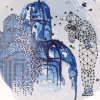
\includegraphics[height=1cm, width=1.5cm]{rbras63.png}%
			%\end{figure}
		%\end{column}\end{columns}}

%\author[Deivison Souza (UFPA)]{\textbf{Deivison Venicio Souza} \\ \scriptsize Doutorando do Programa de Pós-graduação em Engenharia Florestal - UFPR \\ Linha de Pesquisa: Manejo Florestal \\ %(deivisonvs@ufpa.br)}

%\institute[UFPA]{\textbf{Universidade Federal do Pará}}

%\date[\today]{\scriptsize Curitiba, PR \\ \today}

%\titlegraphic{\includegraphics[scale=0.18]{ilogo.png}}
%\logo{\includegraphics[height=1.5cm]{ilogo.png}}

%%%%%%%%%%%%%%%%%%%%%%%%%%%%%%%%%%%%%%%%%%%%%%%%%%%%%%%%%%%%%%%%%%%%%%%%%%%%%%%%%%%%%%%%%%%%%%%%%%%%%%%%%%%%%%%%%%%%%%%%%%
% LÂMINA 1 - INICIO DO DOCUMENTO
%%%%%%%%%%%%%%%%%%%%%%%%%%%%%%%%%%%%%%%%%%%%%%%%%%%%%%%%%%%%%%%%%%%%%%%%%%%%%%%%%%%%%%%%%%%%%%%%%%%%%%%%%%%%%%%%%%%%%%%%%%
\begin{document}

\begin{frame}
 \titlepage
\end{frame}

%%%%%%%%%%%%%%%%%%%%%%%%%%%%%%%%%%%%%%%%%%%%%%%%%%%%%%%%%%%%%%%%%%%%%%%%%%%%%%%%%%%%%%%%%%%%%%%%%%%%%%%%%%%%%%%%%%%%%%%%%%
% LÂMINA 2 - SUMÁRIO
%%%%%%%%%%%%%%%%%%%%%%%%%%%%%%%%%%%%%%%%%%%%%%%%%%%%%%%%%%%%%%%%%%%%%%%%%%%%%%%%%%%%%%%%%%%%%%%%%%%%%%%%%%%%%%%%%%%%%%%%%%

\begin{frame}{Conteúdo}
 \begin{multicols}{2}
  \tableofcontents
 \end{multicols}
\end{frame}

%%%%%%%%%%%%%%%%%%%%%%%%%%%%%%%%%%%%%%%%%%%%%%%%%%%%%%%%%%%%%%%%%%%%%%%%%%%%%%%%%%%%%%%%%%%%%%%%%%%%%%%%%%%%%%%%%%%%%%%%%%
% LÂMINA 3
%%%%%%%%%%%%%%%%%%%%%%%%%%%%%%%%%%%%%%%%%%%%%%%%%%%%%%%%%%%%%%%%%%%%%%%%%%%%%%%%%%%%%%%%%%%%%%%%%%%%%%%%%%%%%%%%%%%%%%%%%%
%\section{A Linguagem R}

%\begin{frame}[t]{A Linguagem R}
	%\transwipe
     %- \textbf{CRAN}: o repositório oficial de pacotes do R;
%\end{frame}

%%%%%%%%%%%%%%%%%%%%%%%%%%%%%%%%%%%%%%%%%%%%%%%%%%%%%%%%%%%%%%%%%%%%%%%%%%%%%%%%%%%%%%%%%%%%%%%%%%%%%%%%%%%%%%%%%%%%%%%%%%
% LÂMINA 3
%%%%%%%%%%%%%%%%%%%%%%%%%%%%%%%%%%%%%%%%%%%%%%%%%%%%%%%%%%%%%%%%%%%%%%%%%%%%%%%%%%%%%%%%%%%%%%%%%%%%%%%%%%%%%%%%%%%%%%%%%%
\begin{frame}[t]{O que é ML?}
	\begin{figure}[H]
		\centering
		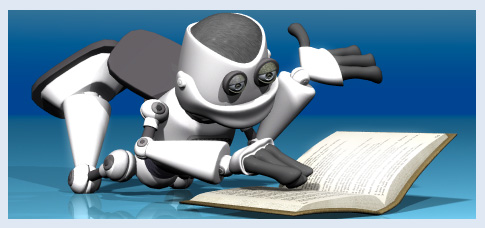
\includegraphics[width=10cm, height=6.5cm]{Fig/maq.jpg}
	\end{figure}
\end{frame}
%%%%%%%%%%%%%%%%%%%%%%%%%%%%%%%%%%%%%%%%%%%%%%%%%%%%%%%%%%%%%%%%%%%%%%%%%%%%%%%%%%%%%%%%%%%%%%%%%%%%%%%%%%%%%%%%%%%%%%%%%%
% LÂMINA 3
%%%%%%%%%%%%%%%%%%%%%%%%%%%%%%%%%%%%%%%%%%%%%%%%%%%%%%%%%%%%%%%%%%%%%%%%%%%%%%%%%%%%%%%%%%%%%%%%%%%%%%%%%%%%%%%%%%%%%%%%%%

\begin{frame}[t]{ML - Definição}
	\transwipe
\textbf{Arthur Lee Samuel:} Termo "Machine Learning" em 1959. \\~\\

\begin{variableblock}{Definição - Parafraseando Samuel (1959)}{bg=white,fg=black}{bg=black,fg=white}
\justifying
\vspace{.5cm}
\large{É um \textcolor{blue}{subconjunto de inteligência artificial} que frequentemente usa técnicas estatísticas para dar aos computadores a capacidade de \textcolor{blue}{''aprender'' com dados}, sem serem explicitamente programados.}

\end{variableblock}

\end{frame}

%%%%%%%%%%%%%%%%%%%%%%%%%%%%%%%%%%%%%%%%%%%%%%%%%%%%%%%%%%%%%%%%%%%%%%%%%%%%%%%%%%%%%%%%%%%%%%%%%%%%%%%%%%%%%%%%%%%%%%%%%%
% LÂMINA 4
%%%%%%%%%%%%%%%%%%%%%%%%%%%%%%%%%%%%%%%%%%%%%%%%%%%%%%%%%%%%%%%%%%%%%%%%%%%%%%%%%%%%%%%%%%%%%%%%%%%%%%%%%%%%%%%%%%%%%%%%%%
%\section{Machine Learning}
%\subsection{Tipos de Aprendizado}

%\begin{frame}[c]{ML - Tipos de Aprendizado}
%	\transwipe

%\begin{tikzpicture}
%\path[mindmap,concept color=green!50!black,text=white]
%node[concept, yscale=.7,xscale=.7] {\LARGE{\textbf{Machine Learning}}}
%child[concept color=red!20, text=black, grow=right,yscale=.9,xscale=.9,level %distance=4cm] {
%	node[concept,yscale=1.3,xscale=1.3] {\small{Unsupervised Learning}}
%	[clockwise from=30]
%	child[level distance=3.4cm] { node[concept color=red!10,yscale=1.3,xscale=1.3] %{\footnotesize{Clustering}} }
%	child[level distance=3.4cm] { node[concept color=red!10,yscale=1.3,xscale=1.3] %{\footnotesize{Association}} }
%}
%child[concept color=blue!20, text=black, grow=left,yscale=.9,xscale=.9,level %distance=4cm] {
%	node[concept,yscale=1.3,xscale=1.3] {\small{Supervised Learning}}
%	[clockwise from=210]
%	child[level distance=3.4cm] { node[concept color=blue!10,yscale=1.3,xscale=1.3] %{\footnotesize{Regression}}
%	}
%	child[level distance=3.4cm] { node[concept color=blue!10,yscale=1.3,xscale=1.3] %{\footnotesize{Classification}}
%}
%}
%;
%\end{tikzpicture}

%\end{frame}

%%%%%%%%%%%%%%%%%%%%%%%%%%%%%%%%%%%%%%%%%%%%%%%%%%%%%%%%%%%%%%%%%%%%%%%%%%%%%%%%%%%%%%%%%%%%%%%%%%%%%%%%%%%%%%%%%%%%%%%%%%
% LÂMINA 5
%%%%%%%%%%%%%%%%%%%%%%%%%%%%%%%%%%%%%%%%%%%%%%%%%%%%%%%%%%%%%%%%%%%%%%%%%%%%%%%%%%%%%%%%%%%%%%%%%%%%%%%%%%%%%%%%%%%%%%%%%%
\section{Machine Learning}

\begin{frame}[c]{Machine Learning}
	\transwipe

\begin{tikzpicture}
\path[mindmap,concept color=green!50!black,text=white]
node[concept, yscale=.7,xscale=.7] {\LARGE{\textbf{Machine Learning}}}
child[concept color=red!20, text=black, grow=right,yscale=.9,xscale=.9,level distance=4cm] {
	node[concept,yscale=1.3,xscale=1.3] {\small{Unsupervised Learning}}
	[clockwise from=30]
	child[level distance=3.2cm] { node[concept color=red!10,yscale=1.3,xscale=1.3] {\small{Clustering}} }
	child[level distance=3.2cm] { node[concept color=red!10,yscale=1.3,xscale=1.3] {\small{Association}} }
}
child[concept color=blue!20, text=black, grow=left,yscale=.9,xscale=.9,level distance=4cm] {
	node[concept,yscale=1.3,xscale=1.3] {\small{Supervised Learning}}
	[clockwise from=210]
	child[level distance=3.2cm] { node[concept color=blue!10,yscale=1.3,xscale=1.3] {\small{Regression}}
	}
	child[level distance=3.2cm] { node[concept color=blue!10,yscale=1.3,xscale=1.3] {\small{Classification}}
}
}
child[concept color=orange!20, text=black, grow=270,yscale=.9,xscale=.9,level distance=4cm] {
	node[concept,yscale=1.2,xscale=1.2] {\small{Semi-supervised Learning}}
	[clockwise from=90]
}
;
\end{tikzpicture}

\end{frame}

%%%%%%%%%%%%%%%%%%%%%%%%%%%%%%%%%%%%%%%%%%%%%%%%%%%%%%%%%%%%%%%%%%%%%%%%%%%%%%%%%%%%%%%%%%%%%%%%%%%%%%%%%%%%%%%%%%%%%%%%%%
% LÂMINA 6
%%%%%%%%%%%%%%%%%%%%%%%%%%%%%%%%%%%%%%%%%%%%%%%%%%%%%%%%%%%%%%%%%%%%%%%%%%%%%%%%%%%%%%%%%%%%%%%%%%%%%%%%%%%%%%%%%%%%%%%%%%

\begin{frame}[t]{Supervised Learning}
	
	\begin{figure}[H]
		\centering
		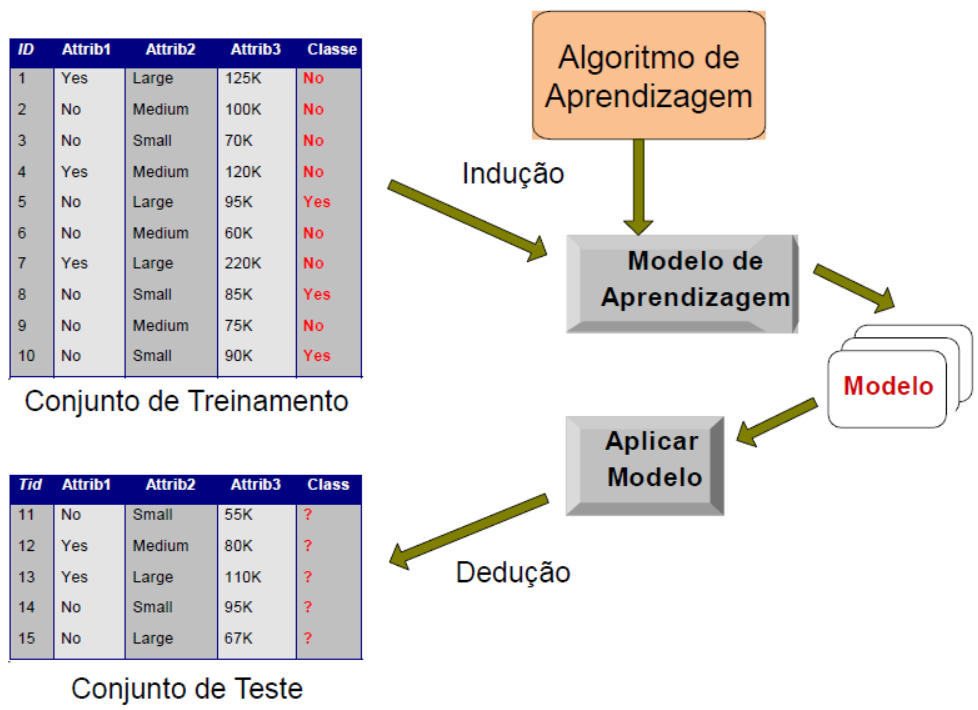
\includegraphics[width=10cm, height=7cm]{Fig/class.png}
	\end{figure}
	
\end{frame}

%%%%%%%%%%%%%%%%%%%%%%%%%%%%%%%%%%%%%%%%%%%%%%%%%%%%%%%%%%%%%%%%%%%%%%%%%%%%%%%%%%%%%%%%%%%%%%%%%%%%%%%%%%%%%%%%%%%%%%%%%%
% LÂMINA 6
%%%%%%%%%%%%%%%%%%%%%%%%%%%%%%%%%%%%%%%%%%%%%%%%%%%%%%%%%%%%%%%%%%%%%%%%%%%%%%%%%%%%%%%%%%%%%%%%%%%%%%%%%%%%%%%%%%%%%%%%%%

\begin{frame}[t]{Estudos}
	
	\begin{figure}[H]
		\centering
		%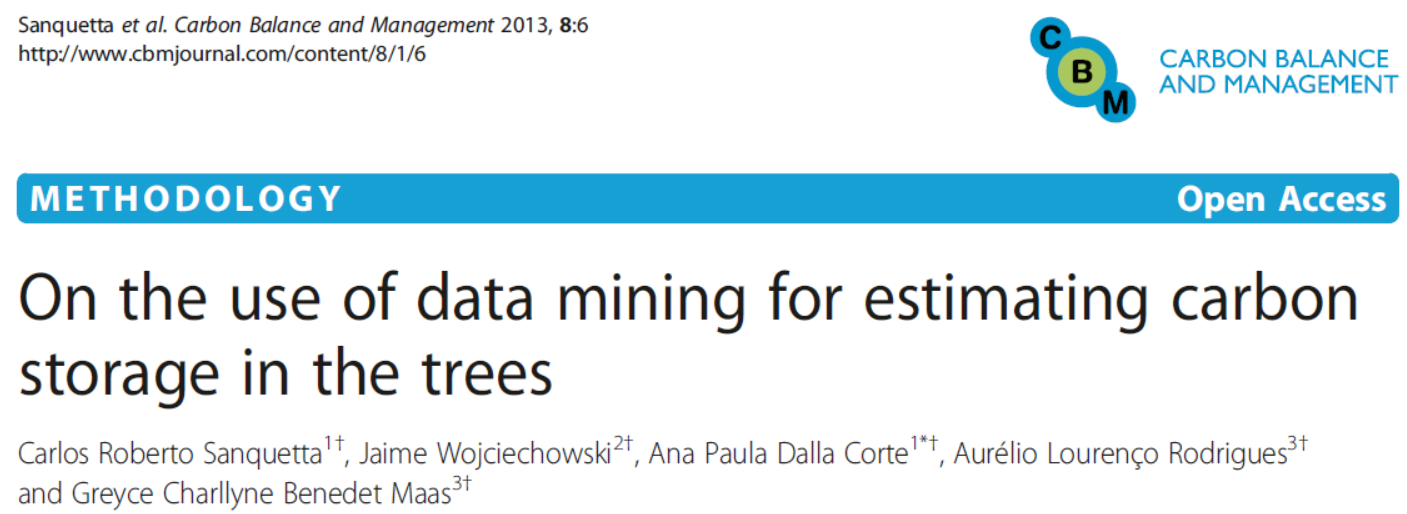
\includegraphics[width=10cm, height=7cm]{Fig/pub1.png}
		%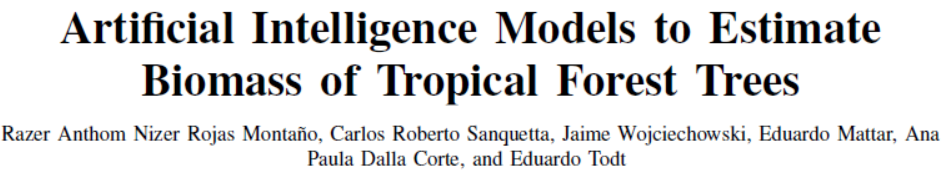
\includegraphics[width=14cm, height=2.5cm]{Fig/Pub2.png}
		
		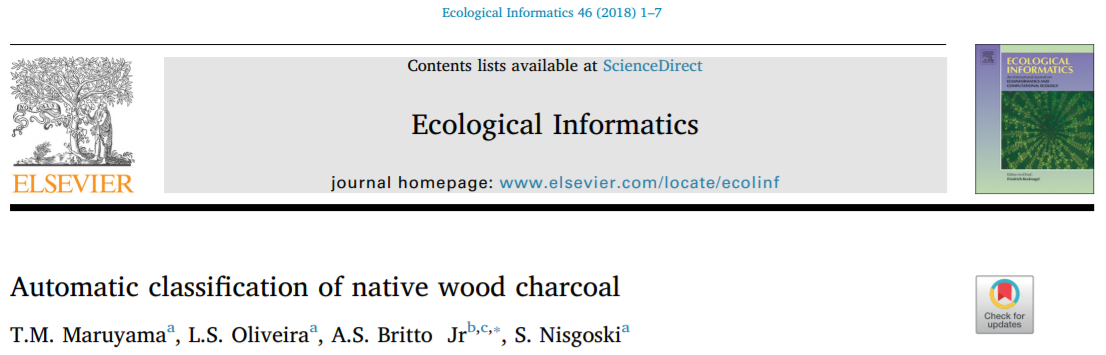
\includegraphics[width=14cm, height=4cm]{Fig/pub3.png}
	\end{figure}
	
\end{frame}

%%%%%%%%%%%%%%%%%%%%%%%%%%%%%%%%%%%%%%%%%%%%%%%%%%%%%%%%%%%%%%%%%%%%%%%%%%%%%%%%%%%%%%%%%%%%%%%%%%%%%%%%%%%%%%%%%%%%%%%%%%
% LÂMINA 6
%%%%%%%%%%%%%%%%%%%%%%%%%%%%%%%%%%%%%%%%%%%%%%%%%%%%%%%%%%%%%%%%%%%%%%%%%%%%%%%%%%%%%%%%%%%%%%%%%%%%%%%%%%%%%%%%%%%%%%%%%%
\begin{frame}[t]{Estudos}
	
	\begin{figure}[H]
		\centering
		%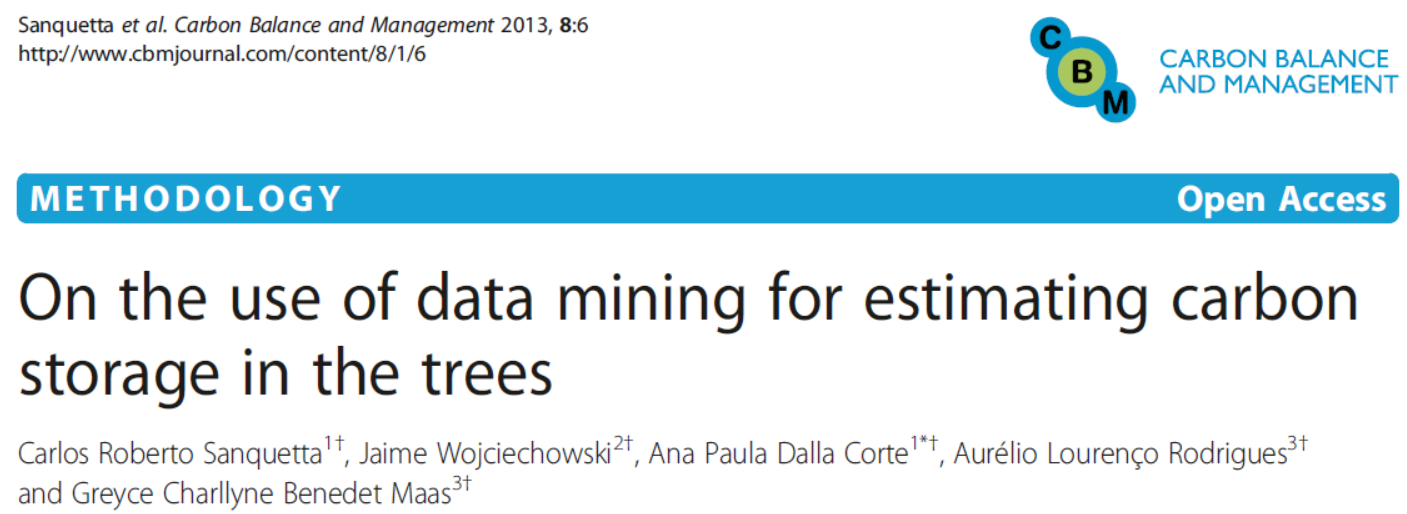
\includegraphics[width=10cm, height=7cm]{Fig/pub1.png}
		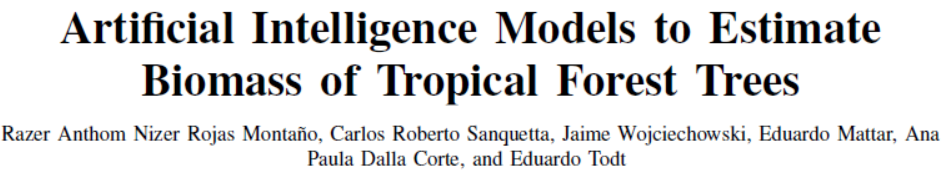
\includegraphics[width=14cm, height=3.5cm]{Fig/Pub2.png}
		
		%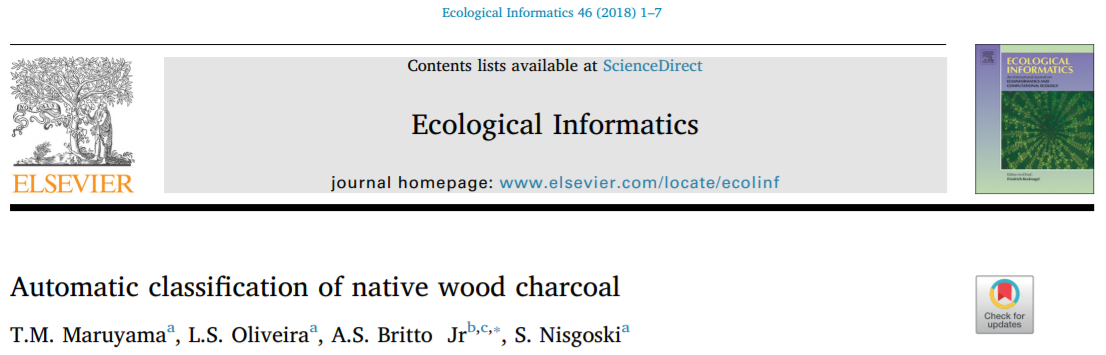
\includegraphics[width=14cm, height=2.5cm]{Fig/pub3.png}
	\end{figure}
	
\end{frame}

%%%%%%%%%%%%%%%%%%%%%%%%%%%%%%%%%%%%%%%%%%%%%%%%%%%%%%%%%%%%%%%%%%%%%%%%%%%%%%%%%%%%%%%%%%%%%%%%%%%%%%%%%%%%%%%%%%%%%%%%%%
% LÂMINA 6
%%%%%%%%%%%%%%%%%%%%%%%%%%%%%%%%%%%%%%%%%%%%%%%%%%%%%%%%%%%%%%%%%%%%%%%%%%%%%%%%%%%%%%%%%%%%%%%%%%%%%%%%%%%%%%%%%%%%%%%%%%
\section{Machine Learning no R}
\subsection{Pacotes disponíveis}

\begin{frame}[t]{CRAN Task View}
	\justifying
	Atualmente, são \textcolor{blue}{102 pacotes} sobre ML publicados no CRAN Task View.
	
	\begin{figure}[H]
		\centering
		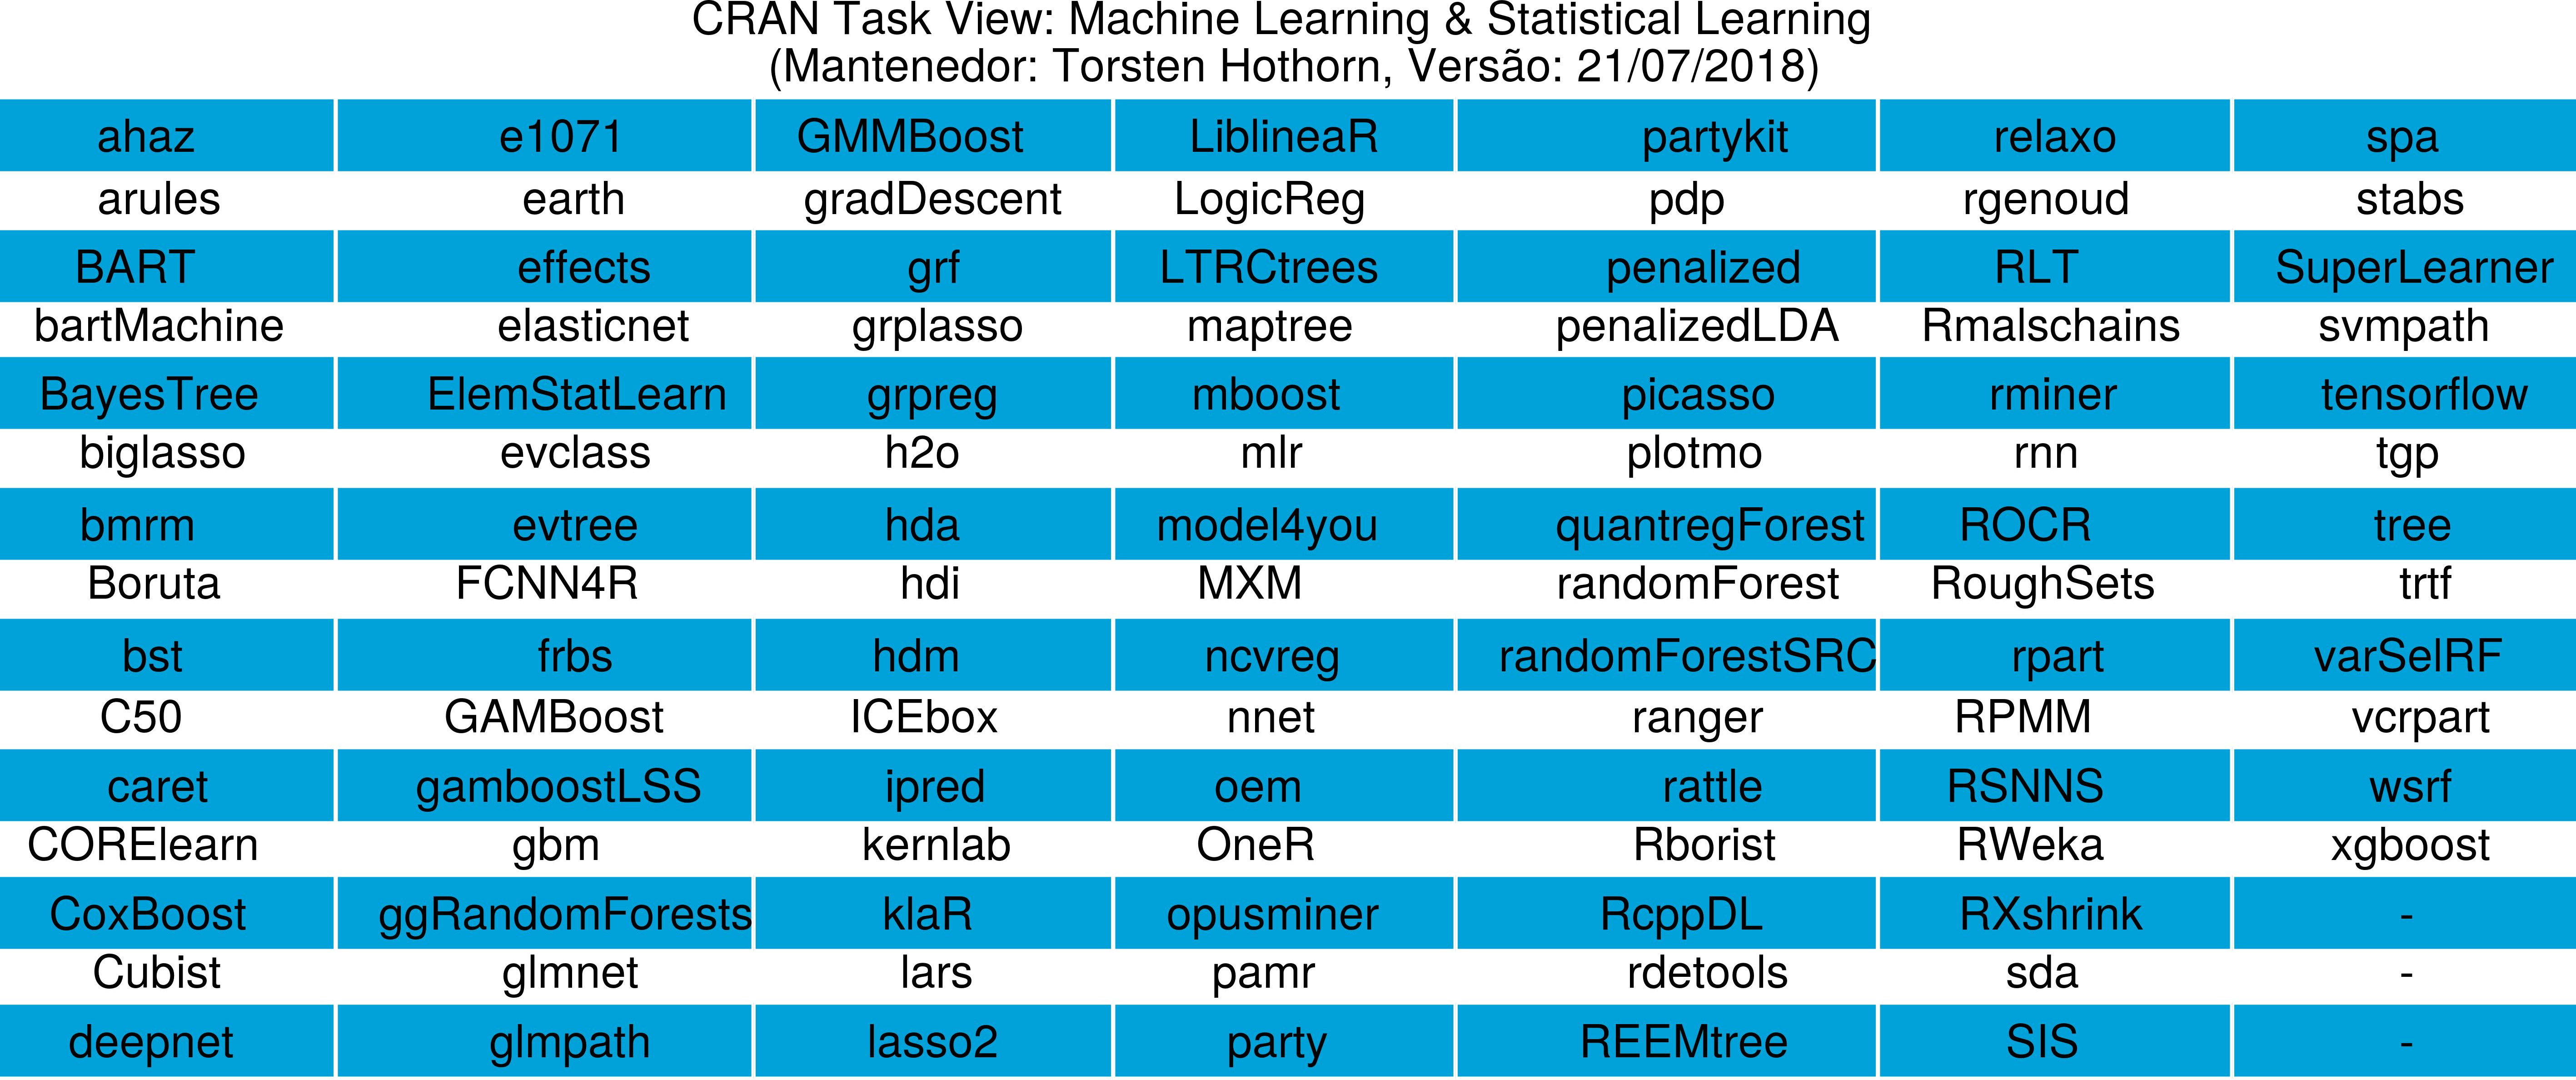
\includegraphics[scale=0.6]{Fig/Task2.jpeg}
	\end{figure}
	
\end{frame}

%%%%%%%%%%%%%%%%%%%%%%%%%%%%%%%%%%%%%%%%%%%%%%%%%%%%%%%%%%%%%%%%%%%%%%%%%%%%%%%%%%%%%%%%%%%%%%%%%%%%%%%%%%%%%%%%%%%%%%%%%%
% LÂMINA 7
%%%%%%%%%%%%%%%%%%%%%%%%%%%%%%%%%%%%%%%%%%%%%%%%%%%%%%%%%%%%%%%%%%%%%%%%%%%%%%%%%%%%%%%%%%%%%%%%%%%%%%%%%%%%%%%%%%%%%%%%%%
\transwipe
\begin{frame}[c]{Qual pacote usar?}

\smartdiagramset{
 planet size=4.5cm,
 planet text width=5cm,
 planet font=\LARGE,
 satellite size=5cm, 
 satellite text width=5cm,
 satellite font=\LARGE,
 distance planet-text=0,
 %distance satellite-text=0,
 distance planet-satellite=6cm,
 /tikz/connection planet satellite/.append style={<-}
 } 
 \begin{center}
 \scalebox{0.4}{
 \smartdiagram[constellation diagram]{
  \textbf{Qual pacote usar?},
  Objetivo,
  Popularidade,
  Número de downloads,
  Tempo de execução}}
  \end{center}

\end{frame}

%%%%%%%%%%%%%%%%%%%%%%%%%%%%%%%%%%%%%%%%%%%%%%%%%%%%%%%%%%%%%%%%%%%%%%%%%%%%%%%%%%%%%%%%%%%%%%%%%%%%%%%%%%%%%%%%%%%%%%%%%%
% LÂMINA 7
%%%%%%%%%%%%%%%%%%%%%%%%%%%%%%%%%%%%%%%%%%%%%%%%%%%%%%%%%%%%%%%%%%%%%%%%%%%%%%%%%%%%%%%%%%%%%%%%%%%%%%%%%%%%%%%%%%%%%%%%%%

\begin{frame}[t]{Qual pacote usar?}
  	
  	\begin{enumerate}
  		\justifying
  		
  		\onslide<2->{\item \textbf{Objetivo}: Qual(is) algoritmo(s) será(ão) testado(s)?;} \newline
  		
  		\onslide<3->{\item \textbf{Popularidade}: Pode-se medir a popularidade dos pacotes de AM;} \newline
  		
  		\onslide<4->{\item \textbf{Número de downloads}: Observar o número de downloads do pacote no repositório CRAN (\textcolor{blue}{pacote cranlogs} $\rightarrow$ \textcolor{magenta}{cran\_downloads()}); e} \newline
  		
  		\onslide<5->{\item \textbf{Tempo de execução}: Maior velocidade de execução da tarefa $\rightarrow$ \textcolor{orange}{Big Data}.}
  		
  	\end{enumerate}
	
\end{frame}

%%%%%%%%%%%%%%%%%%%%%%%%%%%%%%%%%%%%%%%%%%%%%%%%%%%%%%%%%%%%%%%%%%%%%%%%%%%%%%%%%%%%%%%%%%%%%%%%%%%%%%%%%%%%%%%%%%%%%%%%%%
% LÂMINA 8
%%%%%%%%%%%%%%%%%%%%%%%%%%%%%%%%%%%%%%%%%%%%%%%%%%%%%%%%%%%%%%%%%%%%%%%%%%%%%%%%%%%%%%%%%%%%%%%%%%%%%%%%%%%%%%%%%%%%%%%%%%
\subsection{Popularidade de pacotes}

\begin{frame}[t]{TOP 20 - Downloads (últimos 5 ano)}
	
	\begin{figure}[H]
		\centering
		\includegraphics[width=10cm, height=7cm]{Fig/dwl_5year.jpeg}
	\end{figure}
	
\end{frame}

%%%%%%%%%%%%%%%%%%%%%%%%%%%%%%%%%%%%%%%%%%%%%%%%%%%%%%%%%%%%%%%%%%%%%%%%%%%%%%%%%%%%%%%%%%%%%%%%%%%%%%%%%%%%%%%%%%%%%%%%%%
% LÂMINA 9
%%%%%%%%%%%%%%%%%%%%%%%%%%%%%%%%%%%%%%%%%%%%%%%%%%%%%%%%%%%%%%%%%%%%%%%%%%%%%%%%%%%%%%%%%%%%%%%%%%%%%%%%%%%%%%%%%%%%%%%%%%
\begin{frame}[t]{TOP 20 - Downloads (último ano)}
	
	\begin{figure}[H]
		\centering
		\includegraphics[width=10cm, height=7cm]{Fig/dwl_year.jpeg}
	\end{figure}
	
\end{frame}	

%%%%%%%%%%%%%%%%%%%%%%%%%%%%%%%%%%%%%%%%%%%%%%%%%%%%%%%%%%%%%%%%%%%%%%%%%%%%%%%%%%%%%%%%%%%%%%%%%%%%%%%%%%%%%%%%%%%%%%%%%%
% LÂMINA 10
%%%%%%%%%%%%%%%%%%%%%%%%%%%%%%%%%%%%%%%%%%%%%%%%%%%%%%%%%%%%%%%%%%%%%%%%%%%%%%%%%%%%%%%%%%%%%%%%%%%%%%%%%%%%%%%%%%%%%%%%%%
\begin{frame}[t]{TOP 20 - Downloads (30 dias)}
	
	\begin{figure}[H]
		\centering
		\includegraphics[width=10cm, height=7cm]{Fig/dwl_month.jpeg}
	\end{figure}
	
\end{frame}

%%%%%%%%%%%%%%%%%%%%%%%%%%%%%%%%%%%%%%%%%%%%%%%%%%%%%%%%%%%%%%%%%%%%%%%%%%%%%%%%%%%%%%%%%%%%%%%%%%%%%%%%%%%%%%%%%%%%%%%%%%
% LÂMINA 11
%%%%%%%%%%%%%%%%%%%%%%%%%%%%%%%%%%%%%%%%%%%%%%%%%%%%%%%%%%%%%%%%%%%%%%%%%%%%%%%%%%%%%%%%%%%%%%%%%%%%%%%%%%%%%%%%%%%%%%%%%%
%\begin{frame}[t]{Uma inspeção rápida}
	
%\begin{table}[]
	%\centering
	%\begin{tabular}{@{}ll@{}}
		%\toprule
		%\textbf{Pacote}                    & \textbf{Tarefa}  \\ \midrule
		%e1071                              & Divisão de dados \\
		%caret                              & Pré-processamento  \\
		%kernlab                            & Modelagem usando resampling  \\
		%randomForest                       & Configuração de recursos de treino \\
		%rpart                              & Aprendizado dos modelos\\ \bottomrule
	%\end{tabular}
%\end{table}
	
%\end{frame}

%%%%%%%%%%%%%%%%%%%%%%%%%%%%%%%%%%%%%%%%%%%%%%%%%%%%%%%%%%%%%%%%%%%%%%%%%%%%%%%%%%%%%%%%%%%%%%%%%%%%%%%%%%%%%%%%%%%%%%%%%%
% LÂMINA 12
%%%%%%%%%%%%%%%%%%%%%%%%%%%%%%%%%%%%%%%%%%%%%%%%%%%%%%%%%%%%%%%%%%%%%%%%%%%%%%%%%%%%%%%%%%%%%%%%%%%%%%%%%%%%%%%%%%%%%%%%%%
\section{Pacote Caret}

\begin{frame}[c]{}
	
	\begin{center}

	{\Huge \textbf{Pacote} \textcolor{blue}{\textbf{caret}}} \\~\\
	
	{\Large(\textcolor{blue}{\textbf{C}}lassication \textcolor{blue}{\textbf{A}}nd \textcolor{blue}{\textbf{R}}egression \textcolor{blue}{\textbf{T}}raining)} \\~\\
		
	\cite{kuhn2013applied, R-caret} \\~\\

	"Constitui um conjunto de funções que tentam simplificar o processo de construção de modelos preditivos." \\~\\
		
		
	\textbf{web page}: \href{https://topepo.github.io/caret/index.html}{https://topepo.github.io/caret/index.html}
	\end{center}
	
\end{frame}

%%%%%%%%%%%%%%%%%%%%%%%%%%%%%%%%%%%%%%%%%%%%%%%%%%%%%%%%%%%%%%%%%%%%%%%%%%%%%%%%%%%%%%%%%%%%%%%%%%%%%%%%%%%%%%%%%%%%%%%%%%
% LÂMINA 13
%%%%%%%%%%%%%%%%%%%%%%%%%%%%%%%%%%%%%%%%%%%%%%%%%%%%%%%%%%%%%%%%%%%%%%%%%%%%%%%%%%%%%%%%%%%%%%%%%%%%%%%%%%%%%%%%%%%%%%%%%%
%\subsection{Dificuldades ao implementar ML no R}

%\transwipe
%\begin{frame}[t]{Pacote Caret}
%	\textbf{"Dificuldades" ao implementar AM no R:} \newline
	
%	\begin{enumerate}
%	\justifying
	
%	\onslide<2->{\item \textbf{Diferentes contribuidores}: Os pacotes de AM foram %construídos por diversos contribuidores;} \newline
	
%	\onslide<3->{\item \textbf{Diversas funções e pacotes}: Está cada vez mais difícil %acompanhar as nuances sintáticas de cada função dos inúmeros pacotes \cite{Kuhn2008}; %e} \newline
	
%	\onslide<4->{\item \textbf{Testar e comparar vários algoritmos}: Exige o %conhecimento específico de vários pacotes e funções.} \newline
		
%   \end{enumerate}
	
%\end{frame}

%%%%%%%%%%%%%%%%%%%%%%%%%%%%%%%%%%%%%%%%%%%%%%%%%%%%%%%%%%%%%%%%%%%%%%%%%%%%%%%%%%%%%%%%%%%%%%%%%%%%%%%%%%%%%%%%%%%%%%%%%%
% LÂMINA 13
%%%%%%%%%%%%%%%%%%%%%%%%%%%%%%%%%%%%%%%%%%%%%%%%%%%%%%%%%%%%%%%%%%%%%%%%%%%%%%%%%%%%%%%%%%%%%%%%%%%%%%%%%%%%%%%%%%%%%%%%%%
\subsection{Dificuldades ao implementar ML no R}
\transwipe
\begin{frame}[c]{Pacote Caret}

\smartdiagramset{
 planet size=4cm,
 planet text width=5cm,
 planet font=\LARGE,
 satellite size=3.5cm, 
 satellite text width=4cm,
 satellite font=\LARGE,
 distance planet-text=0,
 %distance satellite-text=0,
 distance planet-satellite=7cm,
 /tikz/connection planet satellite/.append style={<-}
 } 
 \begin{center}
 \scalebox{0.4}{
 \smartdiagram[constellation diagram]{
  \textbf{Dificuldades},
  Diferentes contribuidores,
  Diversas funções e pacotes,
  Testar e comparar vários algoritmos}}
  \end{center}

\end{frame}

%%%%%%%%%%%%%%%%%%%%%%%%%%%%%%%%%%%%%%%%%%%%%%%%%%%%%%%%%%%%%%%%%%%%%%%%%%%%%%%%%%%%%%%%%%%%%%%%%%%%%%%%%%%%%%%%%%%%%%%%%%
% LÂMINA 14
%%%%%%%%%%%%%%%%%%%%%%%%%%%%%%%%%%%%%%%%%%%%%%%%%%%%%%%%%%%%%%%%%%%%%%%%%%%%%%%%%%%%%%%%%%%%%%%%%%%%%%%%%%%%%%%%%%%%%%%%%%
%\subsection{Motivação para contruir o caret}

\transwipe
\begin{frame}[t]{Pacote Caret}

	\textbf{O pacote \textcolor{blue}{caret} surge com o objetivo de:} \cite{Kuhn2008} \\~\\
		\justifying
			\onslide<2->{- \textbf{Sintaxe}: Eliminar diferenças sintáticas entre muitas funções de construção de modelos preditivos;} \\~\\
		
			\onslide<3->{- \textbf{Abordagens}: Desenvolver um conjunto de abordagens semi-automatizadas para otimizar os valores de hiperparâmetros de ajuste;} \\~\\
		
			\onslide<4->{- \textbf{Processamento Paralelo}: Criar um pacote que possa ser facilmente estendido para sistemas de processamento paralelo.}
\end{frame}

%%%%%%%%%%%%%%%%%%%%%%%%%%%%%%%%%%%%%%%%%%%%%%%%%%%%%%%%%%%%%%%%%%%%%%%%%%%%%%%%%%%%%%%%%%%%%%%%%%%%%%%%%%%%%%%%%%%%%%%%%%
% LÂMINA 15
%%%%%%%%%%%%%%%%%%%%%%%%%%%%%%%%%%%%%%%%%%%%%%%%%%%%%%%%%%%%%%%%%%%%%%%%%%%%%%%%%%%%%%%%%%%%%%%%%%%%%%%%%%%%%%%%%%%%%%%%%%
%\subsection{Por que usar o caret?}

%\transwipe
%\begin{frame}[t]{Pacote Caret}
	
%	\textbf{Por que usar o pacote \textcolor{blue}{caret}}? \\~\\

%		\justifying
		
%			\onslide<2->{- \textbf{Diferencial}: \textcolor{blue}{Interface uniforme} %para treinamento e previsão de diversos modelos de \textcolor{blue}{aprendizado %supervisionado};} \\~\\
		
%			\onslide<3->{- \textbf{Pacotes já existente}: "Chama" outros pacotes de AM %já existentes para construir os modelos preditivos (com algumas exceções);} \\~\\
		
		%	\onslide<4->{- \textbf{Padronizar tarefas comuns}: %\textcolor{blue}{padroniza as entradas e saídas} no processo de construção dos %modelos;} \\~\\
		
		%	\onslide<5->{- \textbf{Novas funções}: Incorpora e possibilita o uso de %outras funções não disponíveis nos pacotes originais.}
%\end{frame}

%%%%%%%%%%%%%%%%%%%%%%%%%%%%%%%%%%%%%%%%%%%%%%%%%%%%%%%%%%%%%%%%%%%%%%%%%%%%%%%%%%%%%%%%%%%%%%%%%%%%%%%%%%%%%%%%%%%%%%%%%%
% LÂMINA 16
%%%%%%%%%%%%%%%%%%%%%%%%%%%%%%%%%%%%%%%%%%%%%%%%%%%%%%%%%%%%%%%%%%%%%%%%%%%%%%%%%%%%%%%%%%%%%%%%%%%%%%%%%%%%%%%%%%%%%%%%%%

\transwipe
\begin{frame}[c]{Pacote Caret}
\textbf{Por que usar o pacote \textcolor{blue}{caret}}? \\~\\

\smartdiagramset{
 planet size=4cm,
 planet text width=5cm,
 planet font=\LARGE,
 satellite size=3.5cm, 
 satellite text width=4cm,
 satellite font=\LARGE,
 distance planet-text=0,
 %distance satellite-text=0,
 distance planet-satellite=5.3cm,
 /tikz/connection planet satellite/.append style={<-}
 } 
 \begin{center}
 \scalebox{0.4}{
 \smartdiagram[constellation diagram]{
  \textbf{Diferencial},
  Interface uniforme,
  Pacotes já existente,
  Padronizar tarefas comuns,
  Novas funções}}
  \end{center}

\end{frame}

%%%%%%%%%%%%%%%%%%%%%%%%%%%%%%%%%%%%%%%%%%%%%%%%%%%%%%%%%%%%%%%%%%%%%%%%%%%%%%%%%%%%%%%%%%%%%%%%%%%%%%%%%%%%%%%%%%%%%%%%%%
% LÂMINA 16
%%%%%%%%%%%%%%%%%%%%%%%%%%%%%%%%%%%%%%%%%%%%%%%%%%%%%%%%%%%%%%%%%%%%%%%%%%%%%%%%%%%%%%%%%%%%%%%%%%%%%%%%%%%%%%%%%%%%%%%%%%

\transwipe
\begin{frame}[c]{Pacote Caret}
\large{Em termos gerais, o pacote \textcolor{blue}{caret} possui ferramentas para:}

\smartdiagramset{
 planet size=3cm,
 planet text width=3.5cm,
 planet font=\LARGE,
 satellite size=3.5cm, 
 satellite text width=4cm,
 satellite font=\LARGE,
 distance planet-text=0,
 %distance satellite-text=0,
 distance planet-satellite=6cm,
 /tikz/connection planet satellite/.append style={<-}
 } 
 \begin{center}
 \scalebox{0.4}{
 \smartdiagram[constellation diagram]{
  \textbf{Pacote caret},
  Pré-processamento,
  Estimativa de importância das variáveis,
  Ajuste de modelo usando reamostragem,
  Divisão de dados,
  Seleção de recursos}}
  \end{center}

\end{frame}

%%%%%%%%%%%%%%%%%%%%%%%%%%%%%%%%%%%%%%%%%%%%%%%%%%%%%%%%%%%%%%%%%%%%%%%%%%%%%%%%%%%%%%%%%%%%%%%%%%%%%%%%%%%%%%%%%%%%%%%%%%
% LÂMINA 17
%%%%%%%%%%%%%%%%%%%%%%%%%%%%%%%%%%%%%%%%%%%%%%%%%%%%%%%%%%%%%%%%%%%%%%%%%%%%%%%%%%%%%%%%%%%%%%%%%%%%%%%%%%%%%%%%%%%%%%%%%%

\transwipe
\begin{frame}[t]{Pacote Caret}
	\centering
		\begin{tabular}{@{}ll@{}}
			\toprule
			\textbf{Função}                     & \textbf{Tarefa}  \\ \midrule
			findCorrelation()      & Encontrar variáveis altamente correlacionadas \\
			nearZeroVar()          & Identificar preditores com variância próxima de zero \\
			\textcolor{magenta}{preProcess()}           & \textcolor{blue}{Realizar pré-processamento} \\
			\textcolor{magenta}{createDataPartition()}  & \textcolor{blue}{Dividir aleatoriamente o conjunto de dados (estratificação)} \\
			\textcolor{magenta}{train()}                & \textcolor{blue}{Ajustar modelos preditivos utilizando reamostragem} \\ 
			varImp()               & Estimar a importância das variáveis preditoras \\
			resamples()            & Agrupar e visualizar os resultados da reamostragem \\
			diff.resamples()       & Fazer inferências sobre diferenças de desempenho de modelos \\
			confusionMatrix()     & Criar uma matriz de confusão \\
			plotObsVsPred()       & Gerar gráfico de valores observados versus preditos \\ \bottomrule
		\end{tabular}
\end{frame}

%%%%%%%%%%%%%%%%%%%%%%%%%%%%%%%%%%%%%%%%%%%%%%%%%%%%%%%%%%%%%%%%%%%%%%%%%%%%%%%%%%%%%%%%%%%%%%%%%%%%%%%%%%%%%%%%%%%%%%%%%%
%% LÂMINA 17
%%%%%%%%%%%%%%%%%%%%%%%%%%%%%%%%%%%%%%%%%%%%%%%%%%%%%%%%%%%%%%%%%%%%%%%%%%%%%%%%%%%%%%%%%%%%%%%%%%%%%%%%%%%%%%%%%%%%%%%%%%
\section{ML supervisionado}

\begin{frame}[c]{}
	
	\begin{center}
	{\Huge \textbf{Processo SML}} \\[.8em] {\Large \textbf{(Supervised Machine Learning)}} \\[2em]
	
	{\Large Uma abordagem usando o pacote \textcolor{blue}{caret}.} \\[.5em]
	
	\cite{kuhn2013applied, R-caret}
	\end{center}
	
\end{frame}

%%%%%%%%%%%%%%%%%%%%%%%%%%%%%%%%%%%%%%%%%%%%%%%%%%%%%%%%%%%%%%%%%%%%%%%%%%%%%%%%%%%%%%%%%%%%%%%%%%%%%%%%%%%%%%%%%%%%%%%%%%
%% LÂMINA 18
%%%%%%%%%%%%%%%%%%%%%%%%%%%%%%%%%%%%%%%%%%%%%%%%%%%%%%%%%%%%%%%%%%%%%%%%%%%%%%%%%%%%%%%%%%%%%%%%%%%%%%%%%%%%%%%%%%%%%%%%%%	
\begin{frame}[c]{Processo SML - Simplificado}

\tikzstyle{decision} = [diamond, draw, fill=orange!30, 
    text width=4.5em, text badly centered, node distance=3cm, inner sep=0pt]

\tikzstyle{circle1} = [circle, draw, fill=green!20, text centered, radius = 5em]

\tikzstyle{block} = [rectangle, draw, fill=blue!20, 
    text width=6em, text centered, rounded corners, minimum height=4em]
    
\tikzstyle{line} = [draw, -latex']
\tikzstyle{line2} = [draw, -latex',color=red]

\tikzstyle{cloud} = [draw, ellipse,fill=red!20, node distance=3cm,
    minimum height=2em]

\tikzstyle{block1} = [rectangle, draw, fill=red!20, text width=8.3em, text centered, rounded corners, minimum height=1.5em]

\tikzstyle{block2} = [rectangle, draw, fill=red!20, text width=4.5em, text centered, rounded corners, minimum height=1.5em]

\tikzstyle{block3} = [rectangle, draw, fill=blue!20, 
    text width=8em, text centered, rounded corners, minimum height=4em]

\begin{tikzpicture}[node distance = 3.1cm, auto]

% Place nodes
    \node [circle1] (prob) {Problema};
    \node [block, right of=prob] (ide) {Obtenção de dados};
    \node [block, right of=ide] (pre) {Pré-processamento};
    \node [block, right of=pre] (def) {Definição do conjunto de treinamento};
    \node [block, right of=def] (sel) {Seleção de algoritmos};
    \node [block, below of=sel] (treino) {Aprendizado (tuning)};
    \node [block, left of=treino] (teste) {Avaliação no conjunto de teste};
    \node [decision, left of=teste] (dec) {Ok?};
    \node [block, left of=dec] (CR) {Classificador ou Regressor};
    \node [block1, above of=def,node distance=1.5cm] (cdp) {createDataPartition};
    \node [block2, above of=pre,node distance=1.5cm] (preP) {preProcess};
    \node [block2, below of=treino,node distance=1.5cm] (train) {train};
    
% Draw edges
    \path [line] (prob) -- (ide);
    \path [line] (ide) -- (pre);
    \path [line] (pre) -- (def);
    \path [line] (def) -- (sel);
    \path [line] (sel) -- (treino);
    \path [line] (treino) -- (teste);
    \path [line] (teste) -- (dec);
    \path [line] (dec) -- (CR);
    \path [line,dashed] (pre) -- (preP);
    \path [line,dashed] (def) -- (cdp);
    \path [line,dashed] (treino) -- (train);
    \path [line] (dec) -- node[near start]{Sim}(CR);
    \draw[line2,dashed] (dec) to[out=90,in=-90] (ide);
    \path [line2,dashed] (dec) -- node [near start]{Não}(pre);
    \draw[line2,dashed] (dec) to[out=90,in=-90] (def);
    \draw[line2,dashed] (dec) to[out=90,in=-150] (sel);
    
\end{tikzpicture}
\end{frame}

%%%%%%%%%%%%%%%%%%%%%%%%%%%%%%%%%%%%%%%%%%%%%%%%%%%%%%%%%%%%%%%%%%%%%%%%%%%%%%%%%%%%%%%%%%%%%%%%%%%%%%%%%%%%%%%%%%%%%%%%%%
%% LÂMINA 19
%%%%%%%%%%%%%%%%%%%%%%%%%%%%%%%%%%%%%%%%%%%%%%%%%%%%%%%%%%%%%%%%%%%%%%%%%%%%%%%%%%%%%%%%%%%%%%%%%%%%%%%%%%%%%%%%%%%%%%%%%%

\begin{frame}[c]{}
	
	\begin{center}
	{\Huge \textbf{Pré-processamento}} \\~\\
	
	{\LARGE Função preProcess()}
	\end{center}
	
\end{frame}

%%%%%%%%%%%%%%%%%%%%%%%%%%%%%%%%%%%%%%%%%%%%%%%%%%%%%%%%%%%%%%%%%%%%%%%%%%%%%%%%%%%%%%%%%%%%%%%%%%%%%%%%%%%%%%%%%%%%%%%%%%
%% LÂMINA 20
%%%%%%%%%%%%%%%%%%%%%%%%%%%%%%%%%%%%%%%%%%%%%%%%%%%%%%%%%%%%%%%%%%%%%%%%%%%%%%%%%%%%%%%%%%%%%%%%%%%%%%%%%%%%%%%%%%%%%%%%%%
\subsection{Pré-processamento}
\begin{frame}[t]{Pré-processamento}
	
  \begin{variableblock}{Definição}{bg=white,fg=black}{bg=black,fg=white}
	\justifying
	\vspace{.5cm}
	{\large As técnicas de pré-processamento de dados geralmente se referem à \textcolor{blue}{adição}, \textcolor{blue}{exclusão} ou \textcolor{blue}{transformação} dos dados do conjunto de treinamento \cite{kuhn2013applied}, previamente à construção do modelo preditivo.}
  \end{variableblock}

\end{frame}

%%%%%%%%%%%%%%%%%%%%%%%%%%%%%%%%%%%%%%%%%%%%%%%%%%%%%%%%%%%%%%%%%%%%%%%%%%%%%%%%%%%%%%%%%%%%%%%%%%%%%%%%%%%%%%%%%%%%%%%%%%
%% LÂMINA 21
%%%%%%%%%%%%%%%%%%%%%%%%%%%%%%%%%%%%%%%%%%%%%%%%%%%%%%%%%%%%%%%%%%%%%%%%%%%%%%%%%%%%%%%%%%%%%%%%%%%%%%%%%%%%%%%%%%%%%%%%%%
\begin{frame}[t]{Pré-processamento}
	
   \begin{variableblock}{Por que?}{bg=white,fg=black}{bg=black,fg=white}
    \justifying
    \vspace{.5cm}
    \onslide<2->{{\large Os diferentes modelos possuem \textcolor{blue}{sensibilidades distintas} para os tipos de preditores. Assim, a forma com que os preditores entram no modelo também é importante \cite{kuhn2013applied}.}} \\~\\
    
    \onslide<3->{{\large A transformação de preditores é estratégica para diminuir os efeitos de variáveis com \textcolor{blue}{maiores escalas} de medidas sobre a determinação das \textcolor{blue}{métricas de distância} \cite{witten2017data}.}} \\~\\
    
   \end{variableblock}
	
\end{frame}

%%%%%%%%%%%%%%%%%%%%%%%%%%%%%%%%%%%%%%%%%%%%%%%%%%%%%%%%%%%%%%%%%%%%%%%%%%%%%%%%%%%%%%%%%%%%%%%%%%%%%%%%%%%%%%%%%%%%%%%%%%
%% LÂMINA 22
%%%%%%%%%%%%%%%%%%%%%%%%%%%%%%%%%%%%%%%%%%%%%%%%%%%%%%%%%%%%%%%%%%%%%%%%%%%%%%%%%%%%%%%%%%%%%%%%%%%%%%%%%%%%%%%%%%%%%%%%%%
\begin{frame}[t]{Pré-processamento}
	
   \begin{variableblock}{Boa prática?}{bg=white,fg=black}{bg=black,fg=white}
    
    \justifying
    \vspace{.5cm}
    {\large Testar uma série de transformações dos dados brutos combinadas com vários algoritmos de aprendizado de máquina, pode ajudar na descoberta de boas representações dos dados e algoritmos melhores capazes de explorar a estrutura dessas representações (BROWNLEE, 2017).} \\~\\

    {\large \textbf{Algoritmos:} \textit{k}-nearest neighbors, Support Vector Machines, Artificial Neural Networks.}
   \end{variableblock}

\end{frame}

%%%%%%%%%%%%%%%%%%%%%%%%%%%%%%%%%%%%%%%%%%%%%%%%%%%%%%%%%%%%%%%%%%%%%%%%%%%%%%%%%%%%%%%%%%%%%%%%%%%%%%%%%%%%%%%%%%%%%%%%%%
%% LÂMINA 23
%%%%%%%%%%%%%%%%%%%%%%%%%%%%%%%%%%%%%%%%%%%%%%%%%%%%%%%%%%%%%%%%%%%%%%%%%%%%%%%%%%%%%%%%%%%%%%%%%%%%%%%%%%%%%%%%%%%%%%%%%%
\begin{frame}[t]{Pré-processamento}

 \begin{variableblock}{Função preProcess() - métodos}{bg=white,fg=black}{bg=black,fg=white}
    \begin{enumerate}[a)]

     \onslide<2->{\item \textbf{Métodos para padronização ou normalização de variáveis preditoras:}} \\
     
     \onslide<2->{- ”center”: Subtrai cada valor $x_{i}$ da média $\bar{x}$ = ($x_{i}$ - $\bar{x}$).} \\
     \onslide<2->{- ”scale”: Divide cada valor $x_{i}$ pelo desvio padrão $sd_{(x)}$ = ($x_{i}/sd_{(x)})$.} \\
     \onslide<2->{- ”center” e "scale: Padroniza os dados ($\bar{x}$ = 0 e $sd_{(x)}$ = 1).} \\
     \onslide<2->{- "range": Dimensiona os dados no intervalo [0, 1].} \\~\\
     
     \onslide<3->{\item \textbf{Métodos para transformação $\rightarrow$  distribuição mais simétrica:}} \\
     \onslide<3->{- ”BoxCox”: Uma transformação Box-Cox (diferentes de zero e positivos).} \\~\\

    \end{enumerate}\itemsep2pt
 \end{variableblock}
	
\end{frame}

%%%%%%%%%%%%%%%%%%%%%%%%%%%%%%%%%%%%%%%%%%%%%%%%%%%%%%%%%%%%%%%%%%%%%%%%%%%%%%%%%%%%%%%%%%%%%%%%%%%%%%%%%%%%%%%%%
%% LÂMINA 24
%%%%%%%%%%%%%%%%%%%%%%%%%%%%%%%%%%%%%%%%%%%%%%%%%%%%%%%%%%%%%%%%%%%%%%%%%%%%%%%%%%%%%%%%%%%%%%%%%%%%%%%%%%%%%%%%%
\begin{frame}[t]{Pré-processamento}

 \begin{variableblock}{Função preProcess() - métodos}{bg=white,fg=black}{bg=black,fg=white}
    \begin{enumerate}[a)]\setcounter{enumi}{2}

     \onslide<2->{\item \textbf{Métodos de imputação de dados:}} \\
     \justifying
     - "knnImpute": Encontra os k vizinhos mais próximos (euclidiana)  $\rightarrow$ média. \\
     - "medianImpute": Imputação via medianas de cada preditor. \\
     - "bagImpute": Imputação via bagging. \\~\\
     
     \onslide<2->{\item \textbf{Outros métodos:} "YeoJohnson", "expoTrans", "pca", "ica", "spatialSign", "corr", "zv", "nzv", and "conditionalX".} \\~\\
     
     \onslide<3->{Obs.: A função \textcolor{blue}{preProcess} apenas estima os parâmetros necessários para cada método. Em seguida, deve-se usar a função \textcolor{blue}{predict.preProcess} para aplicar o(s) método(s) em conjuntos de dados específicos.}
     
    \end{enumerate}\itemsep2pt
 \end{variableblock}
	
\end{frame}

%%%%%%%%%%%%%%%%%%%%%%%%%%%%%%%%%%%%%%%%%%%%%%%%%%%%%%%%%%%%%%%%%%%%%%%%%%%%%%%%%%%%%%%%%%%%%%%%%%%%%%%%%%%%%%%%%
%% LÂMINA 24
%%%%%%%%%%%%%%%%%%%%%%%%%%%%%%%%%%%%%%%%%%%%%%%%%%%%%%%%%%%%%%%%%%%%%%%%%%%%%%%%%%%%%%%%%%%%%%%%%%%%%%%%%%%%%%%%%
\begin{frame}[t]{Pré-processamento}
\begin{variableblock}{Função preProcess() - Exemplo intuitivo}{bg=white,fg=black}{bg=green!30,fg=black}

	\begin{figure}[H]
		\centering
		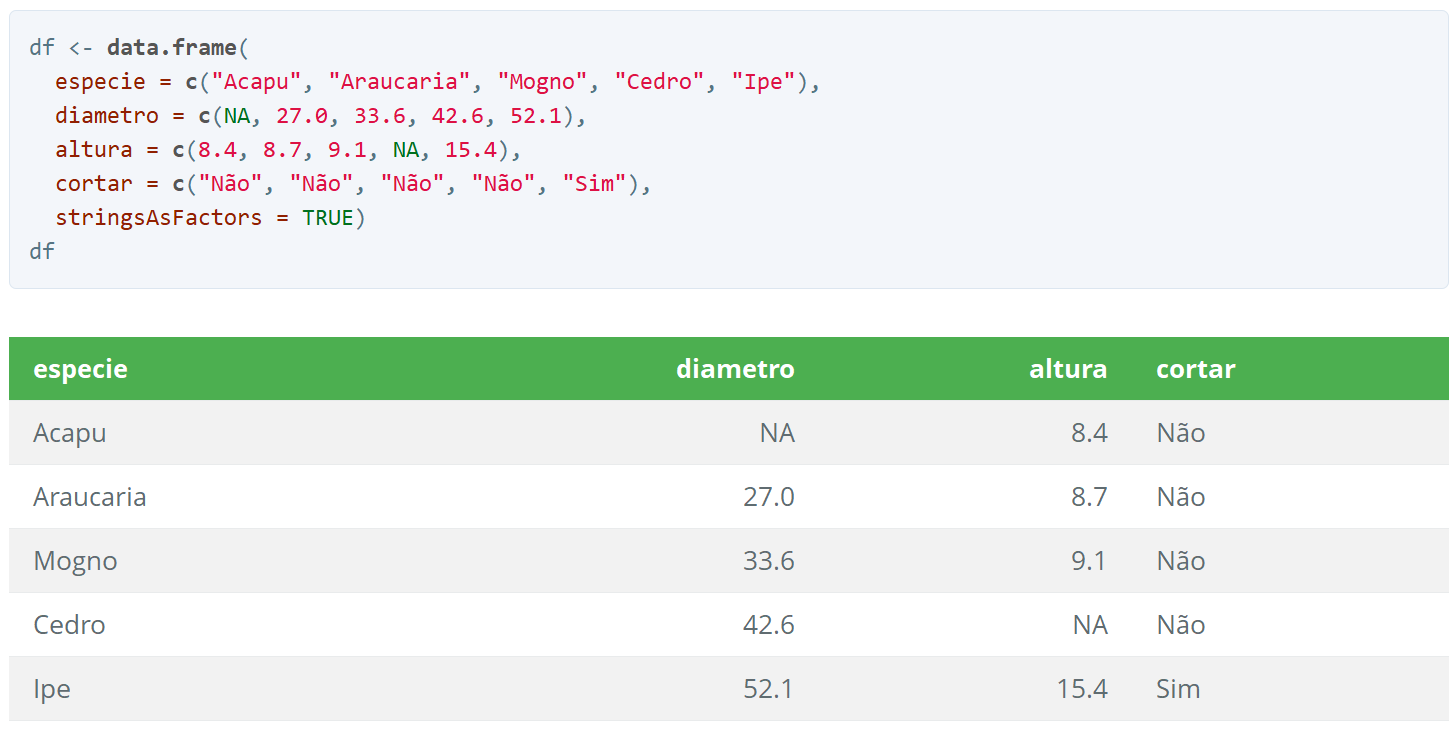
\includegraphics[scale=.35]{Fig/img1.png}
	\end{figure}
	
 \end{variableblock}

\end{frame}

%%%%%%%%%%%%%%%%%%%%%%%%%%%%%%%%%%%%%%%%%%%%%%%%%%%%%%%%%%%%%%%%%%%%%%%%%%%%%%%%%%%%%%%%%%%%%%%%%%%%%%%%%%%%%%%%%
%% LÂMINA 23
%%%%%%%%%%%%%%%%%%%%%%%%%%%%%%%%%%%%%%%%%%%%%%%%%%%%%%%%%%%%%%%%%%%%%%%%%%%%%%%%%%%%%%%%%%%%%%%%%%%%%%%%%%%%%%%%%
\begin{frame}[t]{Pré-processamento}
 \begin{variableblock}{Função preProcess() - "center" $\rightarrow$ "scale"}{bg=white,fg=black}{bg=green!30,fg=black}

	\begin{figure}[H]
		\centering
		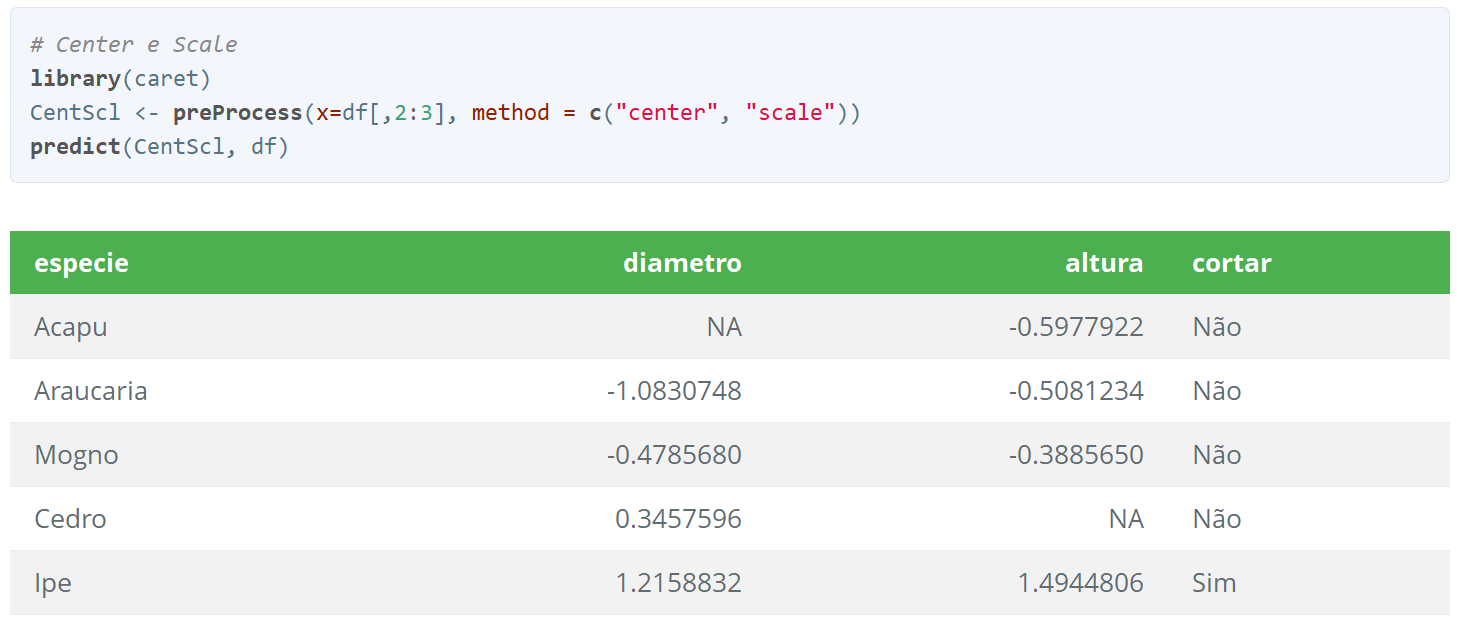
\includegraphics[scale=.35]{Fig/img2.png}
	\end{figure}
	
\end{variableblock}

\end{frame}

%%%%%%%%%%%%%%%%%%%%%%%%%%%%%%%%%%%%%%%%%%%%%%%%%%%%%%%%%%%%%%%%%%%%%%%%%%%%%%%%%%%%%%%%%%%%%%%%%%%%%%%%%%%%%%%%%
%% LÂMINA 24
%%%%%%%%%%%%%%%%%%%%%%%%%%%%%%%%%%%%%%%%%%%%%%%%%%%%%%%%%%%%%%%%%%%%%%%%%%%%%%%%%%%%%%%%%%%%%%%%%%%%%%%%%%%%%%%%%
\begin{frame}[t]{Pré-processamento}
 \begin{variableblock}{Função preProcess() - "center" $\rightarrow$ "scale" $\rightarrow$ "knnImpute"}{bg=white,fg=black}{bg=green!30,fg=black}

	\begin{figure}[H]
		\centering
		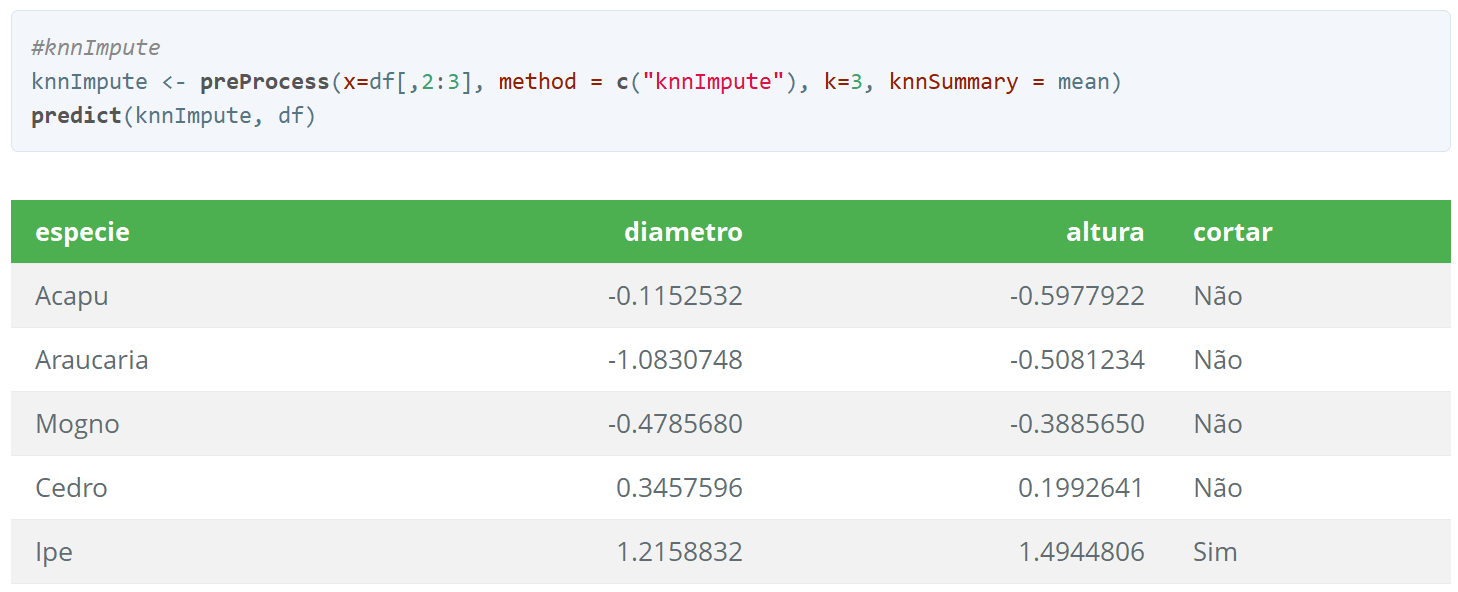
\includegraphics[scale=.35]{Fig/img3.png}
	\end{figure}
	
\end{variableblock}

\end{frame}

%%%%%%%%%%%%%%%%%%%%%%%%%%%%%%%%%%%%%%%%%%%%%%%%%%%%%%%%%%%%%%%%%%%%%%%%%%%%%%%%%%%%%%%%%%%%%%%%%%%%%%%%%%%%%%%%%%%%%%%%%%
%% LÂMINA 25
%%%%%%%%%%%%%%%%%%%%%%%%%%%%%%%%%%%%%%%%%%%%%%%%%%%%%%%%%%%%%%%%%%%%%%%%%%%%%%%%%%%%%%%%%%%%%%%%%%%%%%%%%%%%%%%%%%%%%%%%%%

\begin{frame}[c]{}
	
	\begin{center}
	{\Huge \textbf{Divisão dos dados}} \\~\\
	
	{\LARGE Função createDataPartition()}
	\end{center}
	
\end{frame}

%%%%%%%%%%%%%%%%%%%%%%%%%%%%%%%%%%%%%%%%%%%%%%%%%%%%%%%%%%%%%%%%%%%%%%%%%%%%%%%%%%%%%%%%%%%%%%%%%%%%%%%%%%%%%%%%%
%% LÂMINA 25
%%%%%%%%%%%%%%%%%%%%%%%%%%%%%%%%%%%%%%%%%%%%%%%%%%%%%%%%%%%%%%%%%%%%%%%%%%%%%%%%%%%%%%%%%%%%%%%%%%%%%%%%%%%%%%%%%
\subsection{Divisão dos dados}
\begin{frame}[t]{Divisão dos dados}
 \justifying	
   
    Em geral, em ML reporta-se a três conjuntos de dados \cite{witten2017data}: \\~\\
    
     \textbf{- Conjunto de aprendizado (treino):} Usado para construir os modelos preditivos (classificação ou regressão). \\~\\
     
     \textbf{- Conjunto de validação:} Usado para otimizar os hiperparâmetros dos modelos e escolher a configuração de melhor desempenho preditivo.  \\~\\
     
     \textbf{- Conjunto de teste:} Usado para estimar o desempenho preditivo final do modelo otimizado (\textit{tuning model}).
     
\end{frame}

%%%%%%%%%%%%%%%%%%%%%%%%%%%%%%%%%%%%%%%%%%%%%%%%%%%%%%%%%%%%%%%%%%%%%%%%%%%%%%%%%%%%%%%%%%%%%%%%%%%%%%%%%%%%%%%%%
%% LÂMINA 26
%%%%%%%%%%%%%%%%%%%%%%%%%%%%%%%%%%%%%%%%%%%%%%%%%%%%%%%%%%%%%%%%%%%%%%%%%%%%%%%%%%%%%%%%%%%%%%%%%%%%%%%%%%%%%%%%%
\begin{frame}[t]{Divisão dos dados}
	
 \begin{variableblock}{Importante - Conjuntos independentes}{bg=white,fg=black}{bg=black,fg=white}
    \justifying
    \vspace{.5cm}
    \begin{center}
    \textbf{"Cada um dos três conjuntos deve ser escolhido de forma independente"} \\
     \cite{witten2017data}
    \end{center}
   
    - O conjunto de validação deve ser diferente do conjunto de treinamento para obter um bom desempenho no estágio de otimização ou seleção; e \\~\\
    
    - O conjunto de teste deve ser diferente de ambos para obter uma estimativa confiável da taxa de erro real.
\end{variableblock}

\end{frame}

%%%%%%%%%%%%%%%%%%%%%%%%%%%%%%%%%%%%%%%%%%%%%%%%%%%%%%%%%%%%%%%%%%%%%%%%%%%%%%%%%%%%%%%%%%%%%%%%%%%%%%%%%%%%%%%%%
%% LÂMINA 27
%%%%%%%%%%%%%%%%%%%%%%%%%%%%%%%%%%%%%%%%%%%%%%%%%%%%%%%%%%%%%%%%%%%%%%%%%%%%%%%%%%%%%%%%%%%%%%%%%%%%%%%%%%%%%%%%%
\begin{frame}[t]{Divisão dos dados}
	
 \begin{variableblock}{Função createDataPartition()}{bg=white,fg=black}{bg=black,fg=white}
    \justifying
    \vspace{.5cm}
     A função \textcolor{blue}{createDataPartition} pode ser usada para criar divisões aleatórias estratificadas (\textit{stratified random split}) de um conjunto de dados \cite{Kuhn2008}. \\~\\
     
    \textcolor{blue}{createDataPartition(}y, times = 1, p = 0.5, list = TRUE, groups = min(5,length(y))\textcolor{blue}{)} \\~\\
    
    \textbf{y} = variável que servirá de base para o particionamento. \\
    \textbf{times} = número de partições a serem geradas. \\
    \textbf{p} = porcentagem de dados do conjunto de treinamento. \\
    \textbf{list} = argumento lógico indicando o formato de saída dos resultados. \\
 \end{variableblock}	

\end{frame}

%%%%%%%%%%%%%%%%%%%%%%%%%%%%%%%%%%%%%%%%%%%%%%%%%%%%%%%%%%%%%%%%%%%%%%%%%%%%%%%%%%%%%%%%%%%%%%%%%%%%%%%%%%%%%%%%%
%% LÂMINA 27
%%%%%%%%%%%%%%%%%%%%%%%%%%%%%%%%%%%%%%%%%%%%%%%%%%%%%%%%%%%%%%%%%%%%%%%%%%%%%%%%%%%%%%%%%%%%%%%%%%%%%%%%%%%%%%%%%
\begin{frame}[t]{Divisão dos dados}
	
 \begin{variableblock}{Função createDataPartition()}{bg=white,fg=black}{bg=black,fg=white}
    \justifying
    \vspace{.5cm}
    A amostragem aleatória é feita dentro dos níveis de \textbf{y}: \\~\\
    
    \textbf{Se y = fator}  $\rightarrow$ a amostragem aleatória é feita considerando os níveis de fatores. Assim, busca obter representatividade de todas as classes, bem como equilibrar a quantidade amostrada dentro das classes. \\~\\
    
    \textbf{Se y = numérico}  $\rightarrow$ a amostra é dividida em subgrupos com base em percentis. Assim, a amostragem aleatória é feita dentro desses subgrupos \cite{Kuhn2017}.
    
 \end{variableblock}	
	
\end{frame}

%%%%%%%%%%%%%%%%%%%%%%%%%%%%%%%%%%%%%%%%%%%%%%%%%%%%%%%%%%%%%%%%%%%%%%%%%%%%%%%%%%%%%%%%%%%%%%%%%%%%%%%%%%%%%%%%%
%% LÂMINA 28
%%%%%%%%%%%%%%%%%%%%%%%%%%%%%%%%%%%%%%%%%%%%%%%%%%%%%%%%%%%%%%%%%%%%%%%%%%%%%%%%%%%%%%%%%%%%%%%%%%%%%%%%%%%%%%%%%
\begin{frame}[t]{Divisão dos dados}
 
 \begin{variableblock}{Função createDataPartition() - Iris Flowers Dataset}{bg=white,fg=black}{bg=green!30,fg=black}
 \justifying
    \vspace{-.3cm}
	\begin{figure}[H]
		\centering
		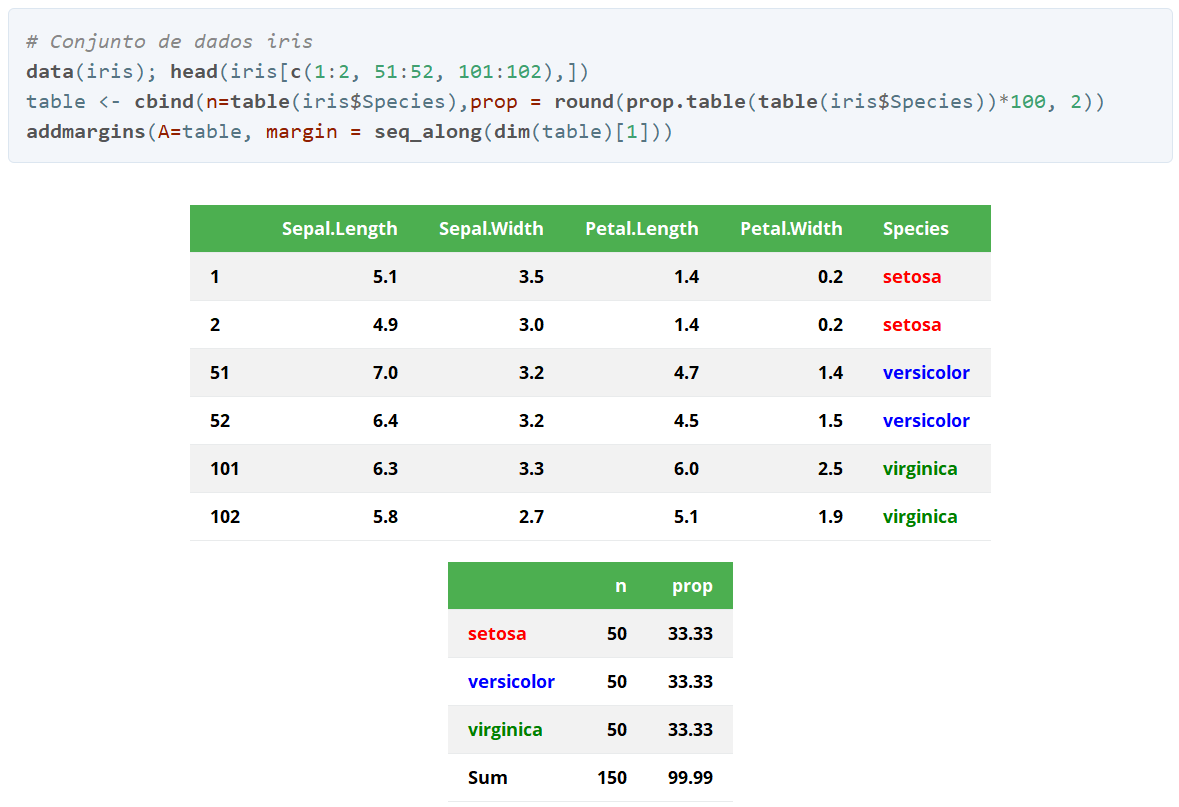
\includegraphics[scale=.35]{Fig/img4.png}
	\end{figure}
 \end{variableblock}
 	
\end{frame}

%%%%%%%%%%%%%%%%%%%%%%%%%%%%%%%%%%%%%%%%%%%%%%%%%%%%%%%%%%%%%%%%%%%%%%%%%%%%%%%%%%%%%%%%%%%%%%%%%%%%%%%%%%%%%%%%%
%% LÂMINA 29
%%%%%%%%%%%%%%%%%%%%%%%%%%%%%%%%%%%%%%%%%%%%%%%%%%%%%%%%%%%%%%%%%%%%%%%%%%%%%%%%%%%%%%%%%%%%%%%%%%%%%%%%%%%%%%%%%
\begin{frame}[t]{Divisão dos dados}
 
 \begin{variableblock}{Função createDataPartition() - Particionando os dados}{bg=white,fg=black}{bg=green!30,fg=black}
 \justifying
    \vspace{-.3cm}
	\begin{figure}[H]
		\centering
		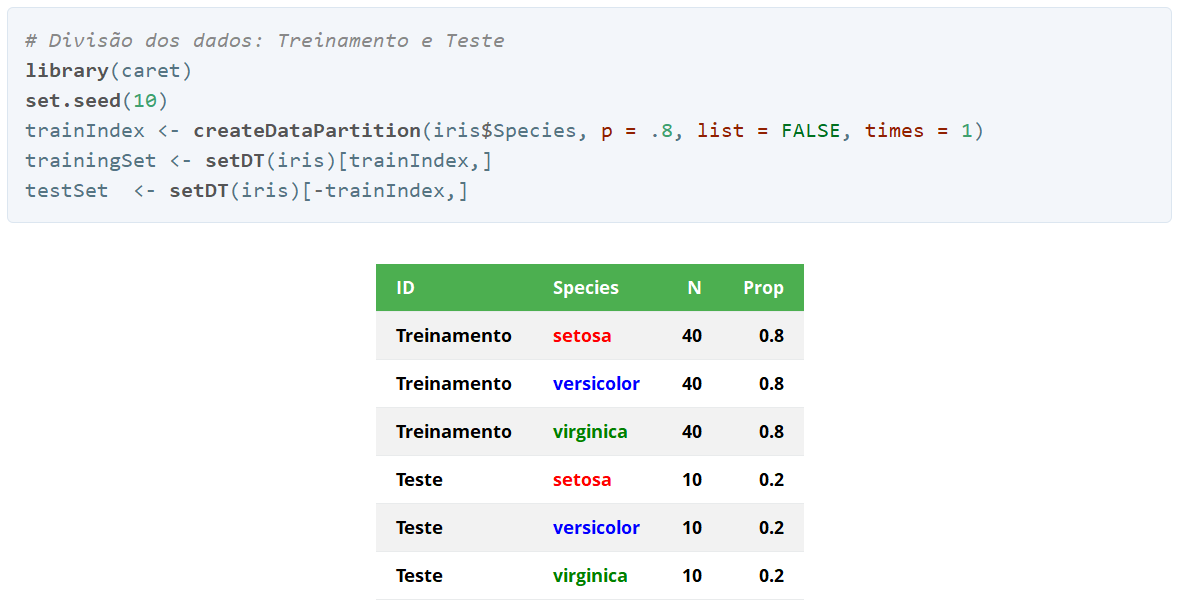
\includegraphics[scale=.4]{Fig/img5.png}
	\end{figure}
 \end{variableblock}
\end{frame}

%%%%%%%%%%%%%%%%%%%%%%%%%%%%%%%%%%%%%%%%%%%%%%%%%%%%%%%%%%%%%%%%%%%%%%%%%%%%%%%%%%%%%%%%%%%%%%%%%%%%%%%%%%%%%%%%%
%% LÂMINA 30
%%%%%%%%%%%%%%%%%%%%%%%%%%%%%%%%%%%%%%%%%%%%%%%%%%%%%%%%%%%%%%%%%%%%%%%%%%%%%%%%%%%%%%%%%%%%%%%%%%%%%%%%%%%%%%%%%
\begin{frame}[t]{Divisão dos dados}
 
 \begin{variableblock}{Função createDataPartition() - Garantia das propriedades estatísticas}{bg=white,fg=black}{bg=green!30,fg=black}
 \justifying
    \vspace{-.3cm}
	\begin{figure}[H]
		\centering
		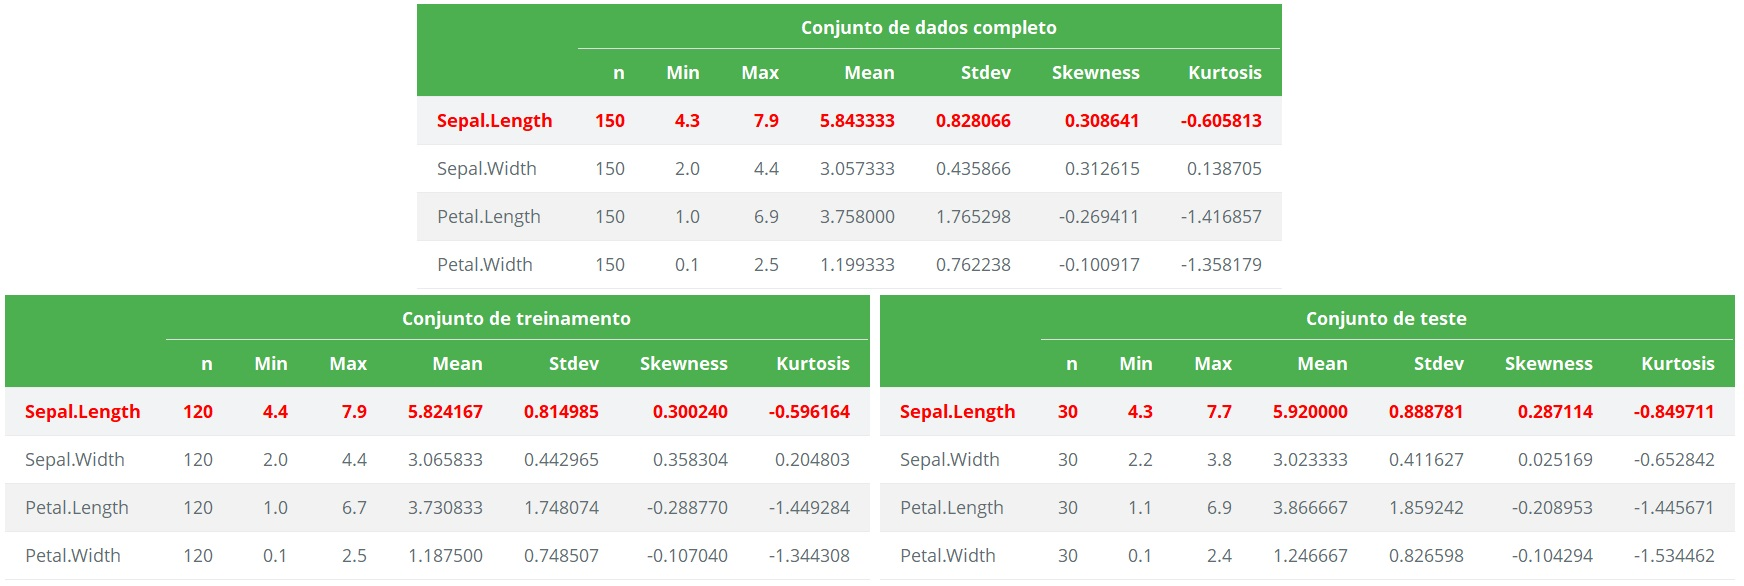
\includegraphics[scale=.38]{Fig/img6.jpg}
	\end{figure}
 \end{variableblock}
\end{frame}

%%%%%%%%%%%%%%%%%%%%%%%%%%%%%%%%%%%%%%%%%%%%%%%%%%%%%%%%%%%%%%%%%%%%%%%%%%%%%%%%%%%%%%%%%%%%%%%%%%%%%%%%%%%%%%%%%
%% LÂMINA 31
%%%%%%%%%%%%%%%%%%%%%%%%%%%%%%%%%%%%%%%%%%%%%%%%%%%%%%%%%%%%%%%%%%%%%%%%%%%%%%%%%%%%%%%%%%%%%%%%%%%%%%%%%%%%%%%%%
%\begin{frame}[t]{Divisão dos dados}
 
 %\begin{variableblock}{Função createDataPartition() - garantia das propriedades %estatísticas}{bg=white,fg=black}{bg=green!30,fg=black}
% \justifying
%    \vspace{.5cm}
 
% De alguma forma a função \textcolor{blue}{createDataPartition()} garante que as %propriedades estatísticas de cada variável, dos conjuntos de aprendizado e teste sejam %semelhantes entre si e equiparáveis ao conjunto de dados completos.
 
% \end{variableblock}

%\end{frame}

%%%%%%%%%%%%%%%%%%%%%%%%%%%%%%%%%%%%%%%%%%%%%%%%%%%%%%%%%%%%%%%%%%%%%%%%%%%%%%%%%%%%%%%%%%%%%%%%%%%%%%%%%%%%%%%%%%%%%%%%%%
%% LÂMINA 31
%%%%%%%%%%%%%%%%%%%%%%%%%%%%%%%%%%%%%%%%%%%%%%%%%%%%%%%%%%%%%%%%%%%%%%%%%%%%%%%%%%%%%%%%%%%%%%%%%%%%%%%%%%%%%%%%%%%%%%%%%%

\begin{frame}[c]{}
	
	\begin{center}
	{\Huge \textbf{Treinamento e Ajuste de Hiperparâmetros}} \\~\\
	
	{\LARGE Função train()}
	\end{center}
	
\end{frame}

%%%%%%%%%%%%%%%%%%%%%%%%%%%%%%%%%%%%%%%%%%%%%%%%%%%%%%%%%%%%%%%%%%%%%%%%%%%%%%%%%%%%%%%%%%%%%%%%%%%%%%%%%%%%%%%%%
%% LÂMINA 32
%%%%%%%%%%%%%%%%%%%%%%%%%%%%%%%%%%%%%%%%%%%%%%%%%%%%%%%%%%%%%%%%%%%%%%%%%%%%%%%%%%%%%%%%%%%%%%%%%%%%%%%%%%%%%%%%%
\subsection{Treinamento e Ajuste de Hiperparâmetros}
\begin{frame}[c]{Treinamento e Ajuste de Hiperparâmetros}
 
 \begin{variableblock}{Hyperparameter}{bg=white,fg=black}{bg=black,fg=white}
  \justifying
    \vspace{.1cm}
Muitos algoritmos de ML possuem "parâmetros" que podem ser ajustados (tuned) para otimizar seu desempenho. Esses parâmetros são denominados \textcolor{blue}{Hiperparâmetros} \cite{witten2017data, probst2018tunability}. \\~\\
\end{variableblock}

 \begin{variableblock}{Hyperparameter tuning}{bg=white,fg=black}{bg=black,fg=white}
 \justifying
    \vspace{.1cm}
 O termo \textcolor{blue}{\textit{hyperparameter tuning}} (hyperparameter optimization) pode ser definido como o processo de encontrar boas configurações de hiperparâmetros de um algoritmo para um conjunto de dados específico \cite{probst2018tunability}.
\end{variableblock}

\end{frame}

%%%%%%%%%%%%%%%%%%%%%%%%%%%%%%%%%%%%%%%%%%%%%%%%%%%%%%%%%%%%%%%%%%%%%%%%%%%%%%%%%%%%%%%%%%%%%%%%%%%%%%%%%%%%%%%%%
%% LÂMINA 32
%%%%%%%%%%%%%%%%%%%%%%%%%%%%%%%%%%%%%%%%%%%%%%%%%%%%%%%%%%%%%%%%%%%%%%%%%%%%%%%%%%%%%%%%%%%%%%%%%%%%%%%%%%%%%%%%%

\begin{frame}[c]{Treinamento e Ajuste de Hiperparâmetros}
 
	\begin{figure}[H]
		\centering
		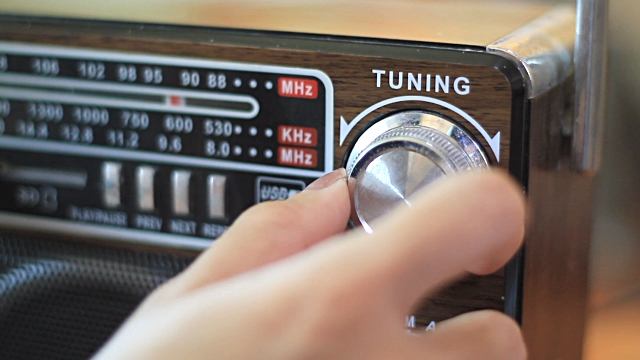
\includegraphics[scale=.6]{Fig/tuning.jpg}
	\end{figure}
	
\end{frame}

%%%%%%%%%%%%%%%%%%%%%%%%%%%%%%%%%%%%%%%%%%%%%%%%%%%%%%%%%%%%%%%%%%%%%%%%%%%%%%%%%%%%%%%%%%%%%%%%%%%%%%%%%%%%%%%%%
%% LÂMINA 33
%%%%%%%%%%%%%%%%%%%%%%%%%%%%%%%%%%%%%%%%%%%%%%%%%%%%%%%%%%%%%%%%%%%%%%%%%%%%%%%%%%%%%%%%%%%%%%%%%%%%%%%%%%%%%%%%%
\begin{frame}[t]{Treinamento e Ajuste de Hiperparâmetros}

Alguns métodos e seus hiperparâmetros de ajuste: \\~\\

\begin{tabular}{@{}lllll@{}}
\toprule
\textbf{Modelo}          & \textbf{Método}   & \textbf{*Tarefa}    & \textbf{Pacote}       & \textbf{Hiperparâmetro} \\ \midrule
k-Nearest Neighbors     & knn               & C, R               & caret        & k                      \\
SVM with Linear Kernel  & svmLinear         & C, R   & kernlab      & C                      \\
SVM with Linear Kernel  & svmLinear2        & C, R   & e1071        & cost                   \\
Multi-Layer Perceptron  & mlp               & C, R   & RSNNS        & size                   \\
Neural Network          & neuralnet         & R      & neuralnet    & layer1,layer2,layer3   \\
Neural Network          & nnet              & C, R   & nnet         & size, decay            \\
Ridge Regression        & ridge             & R      & elasticnet   & lambda                 \\
CART                    & rpart             & C, R   & rpart        & cp                     \\
Random Forest           & rf                & C, R   & randomForest & mtry                   \\ \bottomrule
\end{tabular}
*C = Classificação; R = Regressão
\end{frame}

%%%%%%%%%%%%%%%%%%%%%%%%%%%%%%%%%%%%%%%%%%%%%%%%%%%%%%%%%%%%%%%%%%%%%%%%%%%%%%%%%%%%%%%%%%%%%%%%%%%%%%%%%%%%%%%%%
%% LÂMINA 34
%%%%%%%%%%%%%%%%%%%%%%%%%%%%%%%%%%%%%%%%%%%%%%%%%%%%%%%%%%%%%%%%%%%%%%%%%%%%%%%%%%%%%%%%%%%%%%%%%%%%%%%%%%%%%%%%%
\begin{frame}[t]{Treinamento e Ajuste de Hiperparâmetros}
\begin{variableblock}{Função train()}{bg=white,fg=black}{bg=black,fg=white}
 \justifying
    \vspace{.5cm}
 
 A função \textcolor{blue}{train()} possui as seguintes utilidades: \\~\\
 
 - \textbf{Capacidade preditiva:} Obter a estimativa da capacidade preditiva (performance) para diferentes combinações de hiperparâmetros (candidatos) com base na amostra de treinamento, usando técnicas de reamostragem; e \\~\\
 
- \textbf{Modelo final}: Indicar o melhor modelo preditivo. Isto é, aquele com hiperparâmetros de ajuste ótimo (optimal tuning hyperparameters). Este é o modelo final (tuning model).

 \end{variableblock}
\end{frame}

%%%%%%%%%%%%%%%%%%%%%%%%%%%%%%%%%%%%%%%%%%%%%%%%%%%%%%%%%%%%%%%%%%%%%%%%%%%%%%%%%%%%%%%%%%%%%%%%%%%%%%%%%%%%%%%%%
%% LÂMINA 35
%%%%%%%%%%%%%%%%%%%%%%%%%%%%%%%%%%%%%%%%%%%%%%%%%%%%%%%%%%%%%%%%%%%%%%%%%%%%%%%%%%%%%%%%%%%%%%%%%%%%%%%%%%%%%%%%%
\begin{frame}[t]{Treinamento e Ajuste de Hiperparâmetros}
 \begin{variableblock}{Função train()}{bg=white,fg=black}{bg=black,fg=white}
    \justifying
    \vspace{.5cm}

\textbf{Parâmetros}: \\~\\
- \textbf{x}: matriz ou dataframe que contém as variáveis preditoras; \\
- \textbf{y}: vector que contém a variável de resposta; \\
- \textbf{form}: formula para indicar as variáveis preditoras e a resposta; \\
- \textbf{data}: dataframe que contém o conjunto de dados; \\
- \textbf{method}: método de construção do modelo preditivo (algoritmos); \\ 
- \textbf{preProcess}: pré-processamento das variáveis preditoras; \\
- \textbf{metric}: métrica de avaliação da capacidade preditiva dos modelos ("RMSE", "Rsquared", "Precisão", "ROC"...)

 \end{variableblock}
\end{frame}

%%%%%%%%%%%%%%%%%%%%%%%%%%%%%%%%%%%%%%%%%%%%%%%%%%%%%%%%%%%%%%%%%%%%%%%%%%%%%%%%%%%%%%%%%%%%%%%%%%%%%%%%%%%%%%%%%
%% LÂMINA 34
%%%%%%%%%%%%%%%%%%%%%%%%%%%%%%%%%%%%%%%%%%%%%%%%%%%%%%%%%%%%%%%%%%%%%%%%%%%%%%%%%%%%%%%%%%%%%%%%%%%%%%%%%%%%%%%%%
\begin{frame}[t]{Treinamento e Ajuste de Hiperparâmetros}
 \begin{variableblock}{Função train()}{bg=white,fg=black}{bg=black,fg=white}
    \justifying
    \vspace{.5cm}

\textbf{Parâmetros} (Cont.): \\~\\
- \textbf{trControl}: controlar a construção do modelo e definir a técnica de reamostragem; \\~\\
- \textbf{tuneGrid}: receber um dataframe com os candidatos a hiperparâmetro de ajuste ótimo; e \\~\\
- \textbf{tuneLength}: número de níveis para cada hiperparâmetro de ajuste (usar apenas caso tuneGrid não esteja especificado).

 \end{variableblock}
\end{frame}

%%%%%%%%%%%%%%%%%%%%%%%%%%%%%%%%%%%%%%%%%%%%%%%%%%%%%%%%%%%%%%%%%%%%%%%%%%%%%%%%%%%%%%%%%%%%%%%%%%%%%%%%%%%%%%%%%
%% LÂMINA 35
%%%%%%%%%%%%%%%%%%%%%%%%%%%%%%%%%%%%%%%%%%%%%%%%%%%%%%%%%%%%%%%%%%%%%%%%%%%%%%%%%%%%%%%%%%%%%%%%%%%%%%%%%%%%%%%%%
\begin{frame}[t]{Treinamento e Ajuste de Hiperparâmetros}
 \begin{variableblock}{Função train() - Parâmetro trControl() }{bg=white,fg=black}{bg=black,fg=white}

\begin{center}
\textcolor{blue}{trainControl(}method="repeatedcv",number=10,repeats=10\textcolor{blue}{)}
\end{center}

- \textbf{method}:

\[
\begin{cases}
\boldsymbol{"none"} =~$ajusta um único modelo para todo conj. treino.$ \\
\boldsymbol{"cv"} =~$ k-fold cross-validation.$ \\
\boldsymbol{"repeatedcv"} =~$ repeated k-fold cross-validation.$ \\
\boldsymbol{"boot"} =~$bootstrapping.$ \\
\boldsymbol{"LOOCV"} =~$leave-one-out cross-validation.$ \\
\end{cases}
\] \newline
 \end{variableblock}
\end{frame}

%%%%%%%%%%%%%%%%%%%%%%%%%%%%%%%%%%%%%%%%%%%%%%%%%%%%%%%%%%%%%%%%%%%%%%%%%%%%%%%%%%%%%%%%%%%%%%%%%%%%%%%%%%%%%%%%%
%% LÂMINA 36
%%%%%%%%%%%%%%%%%%%%%%%%%%%%%%%%%%%%%%%%%%%%%%%%%%%%%%%%%%%%%%%%%%%%%%%%%%%%%%%%%%%%%%%%%%%%%%%%%%%%%%%%%%%%%%%%%
\begin{frame}[t]{Treinamento e Ajuste de Hiperparâmetros}
 \begin{variableblock}{Função train() - Esquema de treinamento }{bg=white,fg=black}{bg=black,fg=white}
\begin{figure}[H]
		\centering
		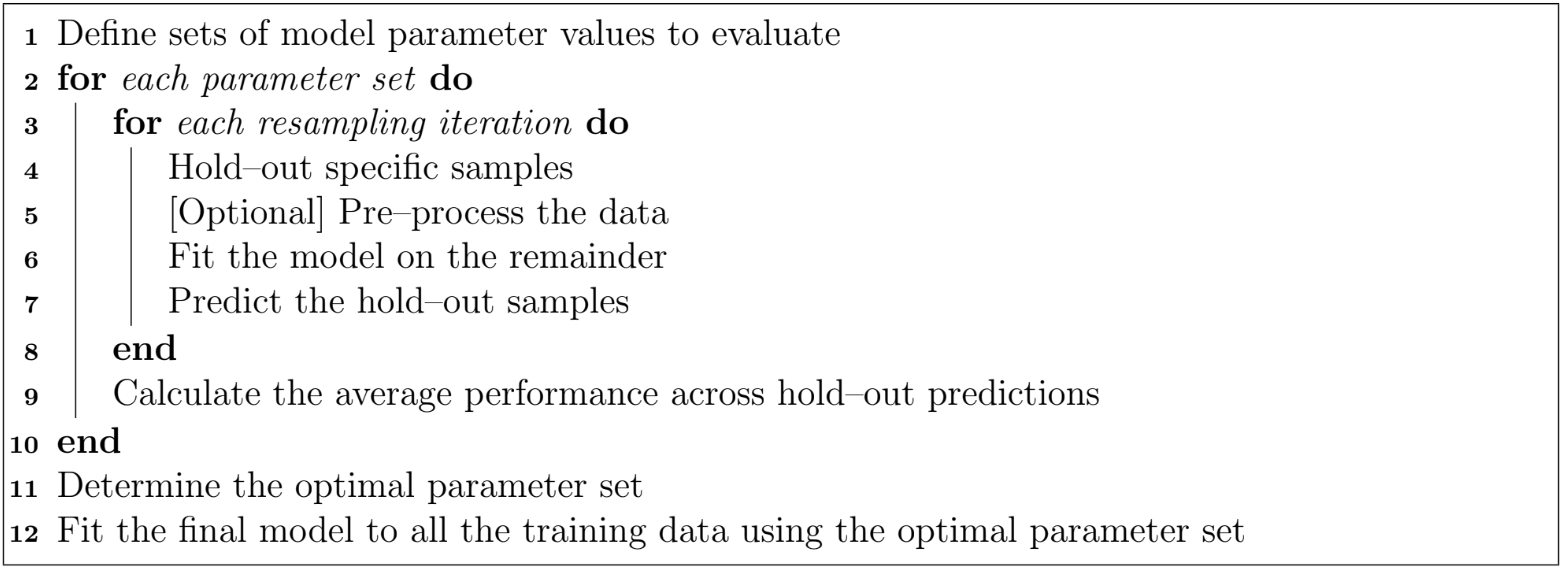
\includegraphics[scale=.42]{Fig/img7.png}
	\end{figure}
	
 \end{variableblock}
\end{frame}

%%%%%%%%%%%%%%%%%%%%%%%%%%%%%%%%%%%%%%%%%%%%%%%%%%%%%%%%%%%%%%%%%%%%%%%%%%%%%%%%%%%%%%%%%%%%%%%%%%%%%%%%%%%%%%%%%
%% LÂMINA 37
%%%%%%%%%%%%%%%%%%%%%%%%%%%%%%%%%%%%%%%%%%%%%%%%%%%%%%%%%%%%%%%%%%%%%%%%%%%%%%%%%%%%%%%%%%%%%%%%%%%%%%%%%%%%%%%%%
\begin{frame}[t]{Treinamento e Ajuste de Hiperparâmetros}

\begin{variableblock}{Métodos de Reamostragem}{bg=white,fg=black}{bg=black,fg=white}
    \justifying
    \vspace{.5cm}
\textbf{- Hold-out validation :}
Separa 2/3 para treinamento e 1/3 para teste. \\~\\

\textbf{- k-fold Cross-Validation:}
Particiona o conj. de treinamento em \textit{k} subconjuntos disjuntos (\textit{k}-1), e testa no conjunto de validação (\textit{hold-out}) (80\%-20\%). \\~\\

\textbf{- Leave-one-out Cross-Validation:} k=n \\~\\

\textbf{- Bootstrap:}
Amostragem com reposição.

\end{variableblock}

\end{frame}

%%%%%%%%%%%%%%%%%%%%%%%%%%%%%%%%%%%%%%%%%%%%%%%%%%%%%%%%%%%%%%%%%%%%%%%%%%%%%%%%%%%%%%%%%%%%%%%%%%%%%%%%%%%%%%%%%
%% LÂMINA 38
%%%%%%%%%%%%%%%%%%%%%%%%%%%%%%%%%%%%%%%%%%%%%%%%%%%%%%%%%%%%%%%%%%%%%%%%%%%%%%%%%%%%%%%%%%%%%%%%%%%%%%%%%%%%%%%%%

\begin{frame}[c]

\begin{center}

 \Large{\textcolor{blue}{\textbf{Navalha de Occam}}} (Guilherme de Occam) \\~\\
 
\textbf{Dados dois modelos com erro de generalização similares, deve-se preferir o modelo mais simples em relação ao modelo mais complexo.}
\end{center}

\end{frame}

%%%%%%%%%%%%%%%%%%%%%%%%%%%%%%%%%%%%%%%%%%%%%%%%%%%%%%%%%%%%%%%%%%%%%%%%%%%%%%%%%%%%%%%%%%%%%%%%%%%%%%%%%%%%%%%%%
%% LÂMINA 38
%%%%%%%%%%%%%%%%%%%%%%%%%%%%%%%%%%%%%%%%%%%%%%%%%%%%%%%%%%%%%%%%%%%%%%%%%%%%%%%%%%%%%%%%%%%%%%%%%%%%%%%%%%%%%%%%%

%\begin{frame}[c]

%\begin{center}
%\Large{\textit{k}-nearest neighbor regression in the estimation of \textit{T. grandis} %stem volume in Pará, Brazil.} \textbf{(Em revisão)} \\~\\

% \Large{\textcolor{blue}{“Me diga com quem tu andas e eu direi quem tu és”!}}
%\end{center}

%\end{frame}

%%%%%%%%%%%%%%%%%%%%%%%%%%%%%%%%%%%%%%%%%%%%%%%%%%%%%%%%%%%%%%%%%%%%%%%%%%%%%%%%%%%%%%%%%%%%%%%%%%%%%%%%%%%%%%%%%
%% LÂMINA 39
%%%%%%%%%%%%%%%%%%%%%%%%%%%%%%%%%%%%%%%%%%%%%%%%%%%%%%%%%%%%%%%%%%%%%%%%%%%%%%%%%%%%%%%%%%%%%%%%%%%%%%%%%%%%%%%%%

%\begin{frame}[t]

% \begin{variableblock}{Configuração do treinamento} %{bg=white,fg=black}{bg=black,fg=white}
%	Variação = preditores
%	preProcess = "center" e "scale" \\~\\
%	method = "knn" \\~\\
%	metric = "RMSE" \\~\\
%	tuneGrid = (k = seq(3, 25, by = 2)) \\~\\
%	trainControl(method="repeatedcv",number=10,repeats=3)
% \end{variableblock}

%\end{frame}

%%%%%%%%%%%%%%%%%%%%%%%%%%%%%%%%%%%%%%%%%%%%%%%%%%%%%%%%%%%%%%%%%%%%%%%%%%%%%%%%%%%%%%%%%%%%%%%%%%%%%%%%%%%%%%%%%
%% LÂMINA 39
%%%%%%%%%%%%%%%%%%%%%%%%%%%%%%%%%%%%%%%%%%%%%%%%%%%%%%%%%%%%%%%%%%%%%%%%%%%%%%%%%%%%%%%%%%%%%%%%%%%%%%%%%%%%%%%%%

%\begin{frame}[c]

% \begin{variableblock}{Estimativa de desempenho sob 3x10-folds CV em função de k.} %{bg=white,fg=black}{bg=black,fg=white}

%	\begin{figure}[H]
%		\centering
%		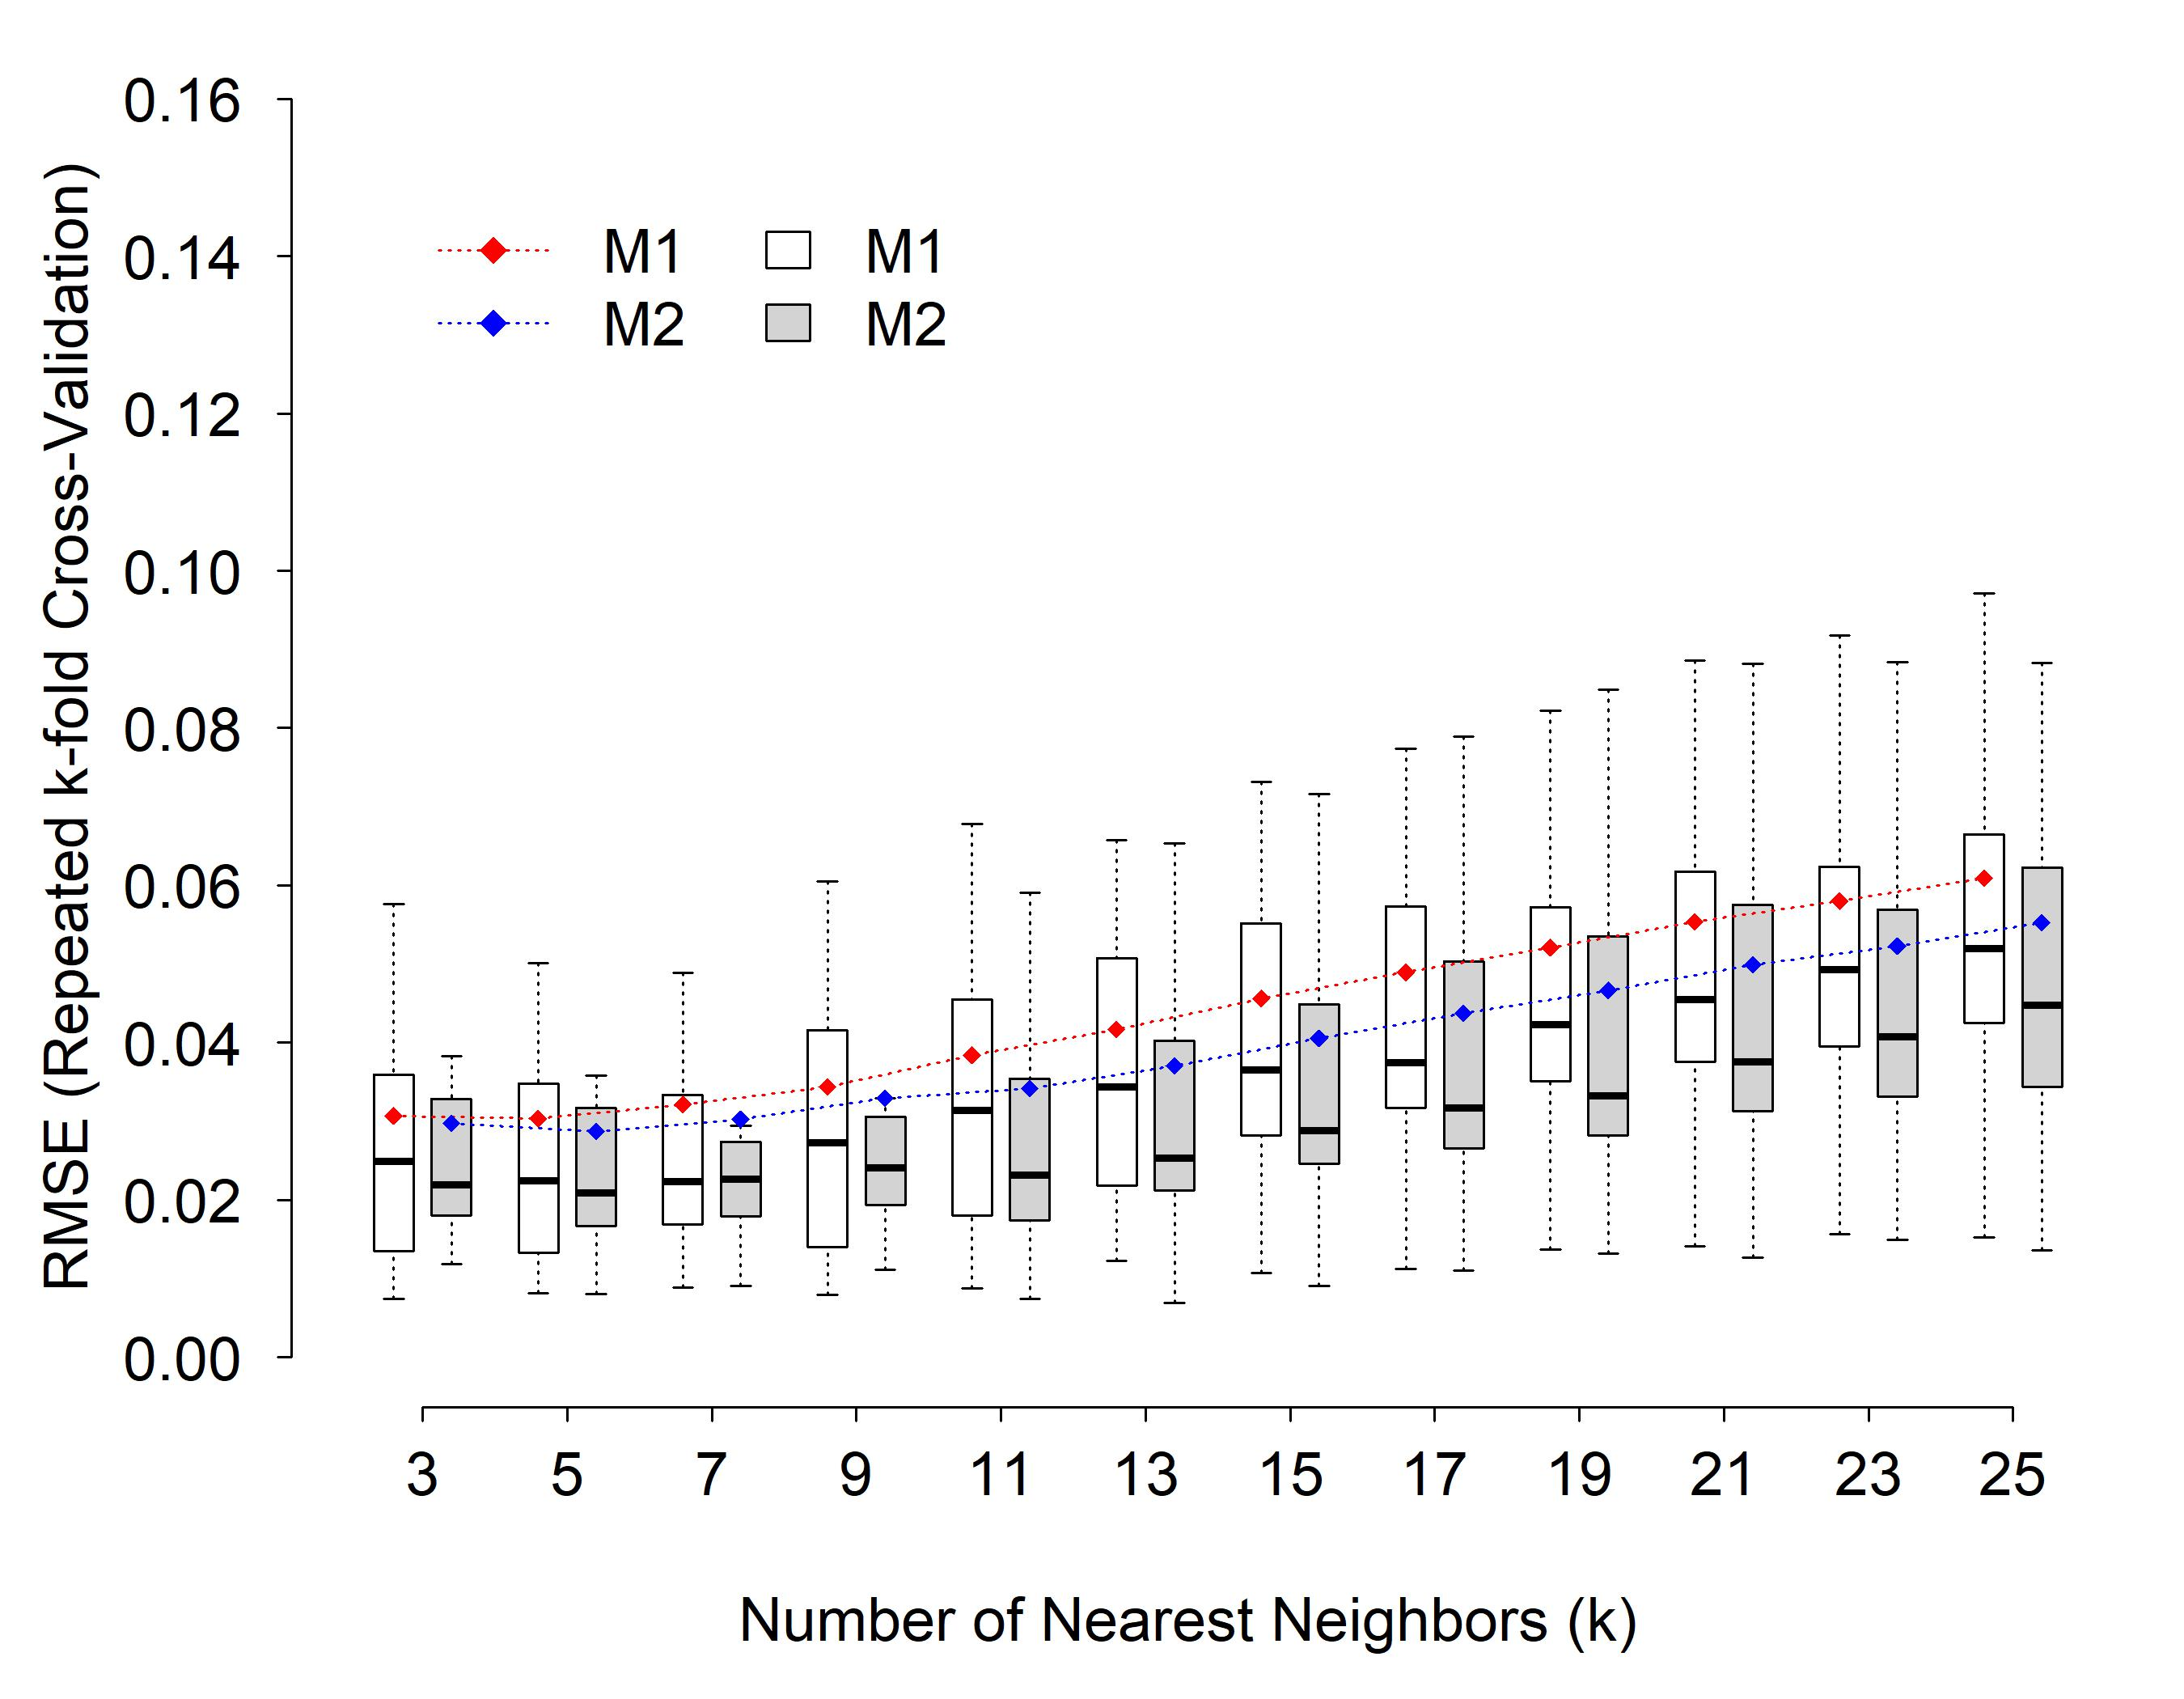
\includegraphics[height=7cm, width=12cm]{Fig/Figure2.jpeg}
%	\end{figure}
	
% \end{variableblock}

%\end{frame}

%%%%%%%%%%%%%%%%%%%%%%%%%%%%%%%%%%%%%%%%%%%%%%%%%%%%%%%%%%%%%%%%%%%%%%%%%%%%%%%%%%%%%%%%%%%%%%%%%%%%%%%%%%%%%%%%%
%% LÂMINA 39
%%%%%%%%%%%%%%%%%%%%%%%%%%%%%%%%%%%%%%%%%%%%%%%%%%%%%%%%%%%%%%%%%%%%%%%%%%%%%%%%%%%%%%%%%%%%%%%%%%%%%%%%%%%%%%%%%

%\begin{frame}[c]

% \begin{variableblock}{Estimativa de desempenho sob 3x10-folds CV em função de k.} %{bg=white,fg=black}{bg=black,fg=white}

	%\begin{figure}[H]
		%\centering
		%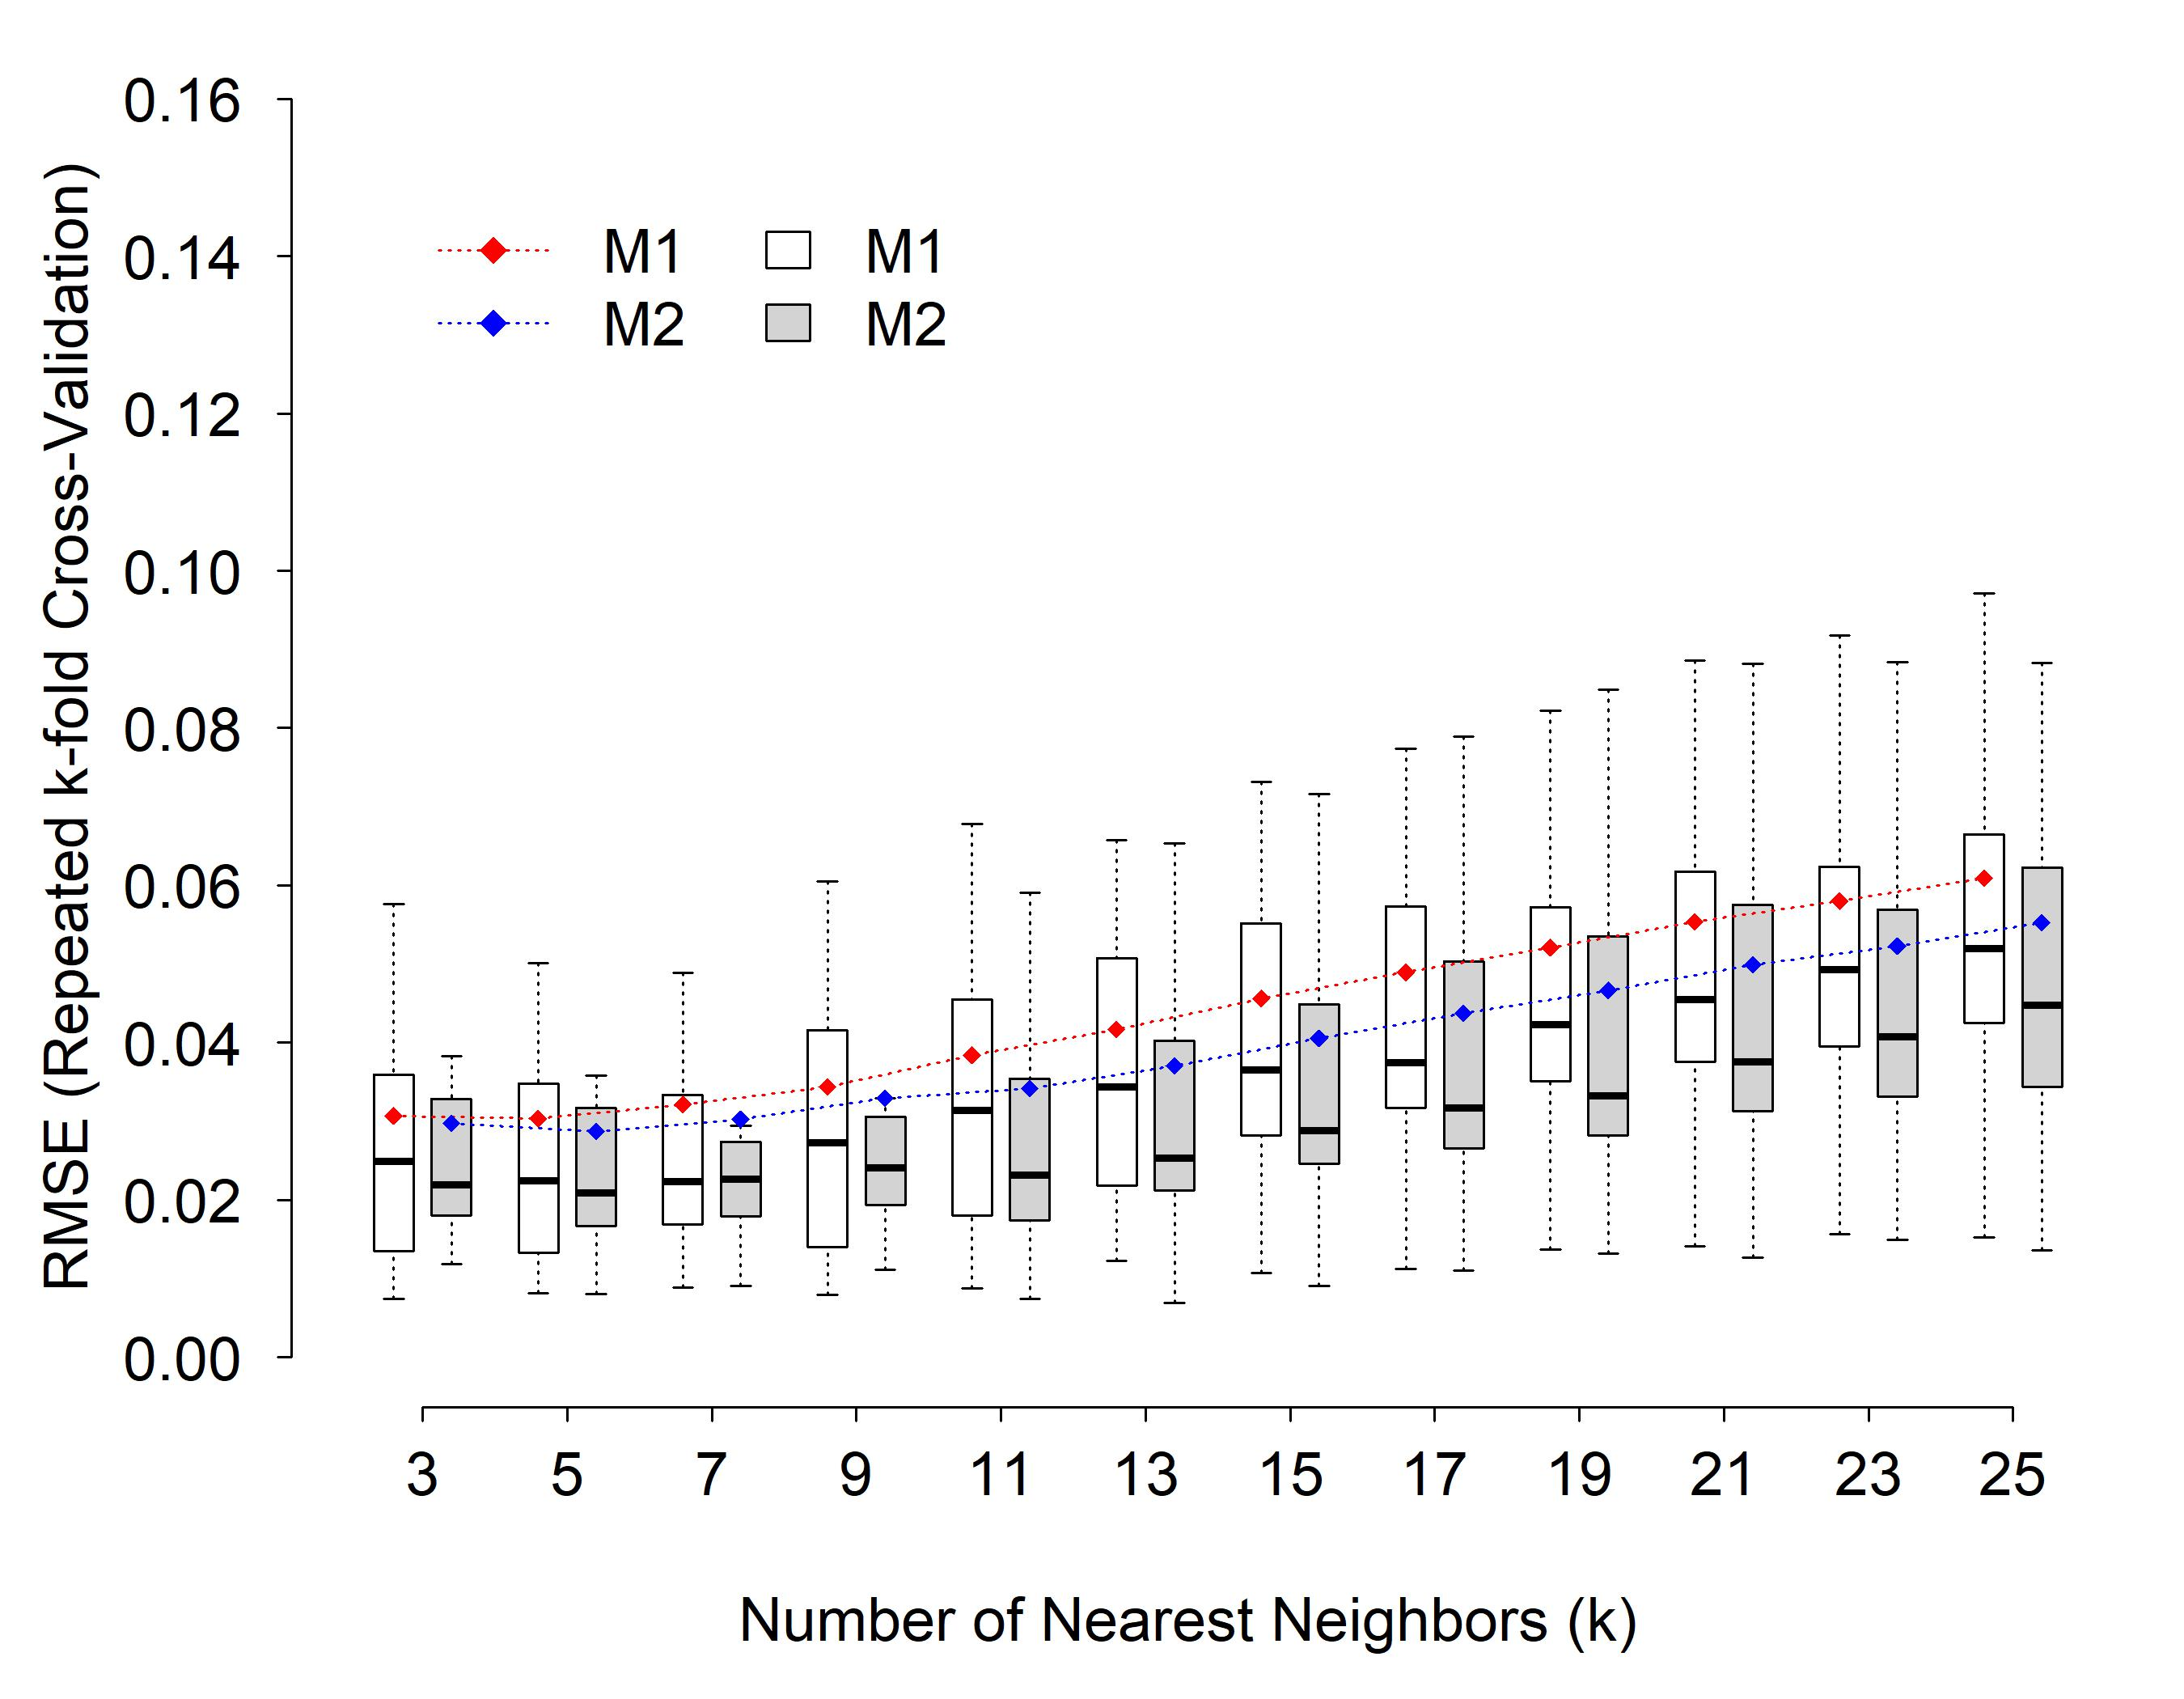
\includegraphics[height=7cm, width=12cm]{Fig/Figure2.jpeg}
	%\end{figure}
	
 %\end{variableblock}

%\end{frame}

%%%%%%%%%%%%%%%%%%%%%%%%%%%%%%%%%%%%%%%%%%%%%%%%%%%%%%%%%%%%%%%%%%%%%%%%%%%%%%%%%%%%%%%%%%%%%%%%%%%%%%%%%%%%%%%%%
%% LÂMINA 40
%%%%%%%%%%%%%%%%%%%%%%%%%%%%%%%%%%%%%%%%%%%%%%%%%%%%%%%%%%%%%%%%%%%%%%%%%%%%%%%%%%%%%%%%%%%%%%%%%%%%%%%%%%%%%%%%%
%\begin{frame}[t]{Treinamento e Ajuste de Hiperparâmetros}
% \begin{variableblock}{Função train() - Esquema de treinamento %}{bg=white,fg=black}{bg=black,fg=white}
%- Overfitting significa que o modelo tem um bom desempenho nos dados de treinamento, %mas não é generalizado.
% \end{variableblock}
%\end{frame}

%%%%%%%%%%%%%%%%%%%%%%%%%%%%%%%%%%%%%%%%%%%%%%%%%%%%%%%%%%%%%%%%%%%%%%%%%%%%%%%%%%%%%%%%%%%%%%%%%%%%%%%%%%%%%%%%%
%% LÂMINA 41
%%%%%%%%%%%%%%%%%%%%%%%%%%%%%%%%%%%%%%%%%%%%%%%%%%%%%%%%%%%%%%%%%%%%%%%%%%%%%%%%%%%%%%%%%%%%%%%%%%%%%%%%%%%%%%%%%



%%%%%%%%%%%%%%%%%%%%%%%%%%%%%%%%%%%%%%%%%%%%%%%%%%%%%%%%%%%%%%%%%%%%%%%%%%%%%%%%%%%%%%%%%%%%%%%%%%%%%%%%%%%%%%%%%
%% LÂMINA 42
%%%%%%%%%%%%%%%%%%%%%%%%%%%%%%%%%%%%%%%%%%%%%%%%%%%%%%%%%%%%%%%%%%%%%%%%%%%%%%%%%%%%%%%%%%%%%%%%%%%%%%%%%%%%%%%%%

%\begin{frame}[c]{Movie}

%  \centering 
% 	\movie[height = 7.5cm, width = 7.5cm]{}{Vid/KfCV.mp4}
% \movie{\includegraphics[height = 6.5cm, width = 8.0cm]{Fig/dwl_5year.jpeg}}{Vid/KfCV.mp4}

%\end{frame}

%\begin{frame}[]{Movie}

%\begin{center}
%\includemedia[
%width = 7.5cm,height = 7.5cm,
%addresource = Vid/KfCV.mp4,
%transparent,
%activate = pageopen,
%passcontext,
%flashvars = {
%source = Vid/KfCV.mp4
%&autoPlay = false
%&loop = true
%}
%]{}{VPlayer.swf}
%\end{center}

%\end{frame}

%%%%%%%%%%%%%%%%%%%%%%%%%%%%%%%%%%%%%%%%%%%%%%%%%%%%%%%%%%%%%%%%%%%%%%%%%%%%%%%%%%%%%%%%%%%%%%%%%%%%%%%%%%%%%%%%%%%%%%%%%%
%% LÂMINA 43
%%%%%%%%%%%%%%%%%%%%%%%%%%%%%%%%%%%%%%%%%%%%%%%%%%%%%%%%%%%%%%%%%%%%%%%%%%%%%%%%%%%%%%%%%%%%%%%%%%%%%%%%%%%%%%%%%%%%%%%%%%
%\begin{frame}
	%\frametitle{Youtube video}
	%\includemedia[
	%width=7.11cm,height=4cm,
	%activate=pageopen,
	%flashvars={
		%modestbranding=1 % no YT logo in control bar
		%&autohide=1 % controlbar autohide
		%&showinfo=0 % no title and other info before start
		%&rel=0 % no related videos after end
	%},
	%url % Flash loaded from URL
	%]{}{https://www.youtube.com/watch?v=ADNFKiAjmWA}
%\end{frame}

%%%%%%%%%%%%%%%%%%%%%%%%%%%%%%%%%%%%%%%%%%%%%%%%%%%%%%%%%%%%%%%%%%%%%%%%%%%%%%%%%%%%%%%%%%%%%%%%%%%%%%%%%%%%%%%%%
%% CONSIDERAÇÕES FINAIS
%%%%%%%%%%%%%%%%%%%%%%%%%%%%%%%%%%%%%%%%%%%%%%%%%%%%%%%%%%%%%%%%%%%%%%%%%%%%%%%%%%%%%%%%%%%%%%%%%%%%%%%%%%%%%%%%%
\begin{frame}[t]{Considerações Finais}

	\begin{variableblock}{Desafios}{bg=white,fg=black}{bg=black,fg=white}
	\justifying
	\textcolor{blue}{Compreender melhor e avançar} nas implementações de tarefas de ML nas Ciências Florestais! \\~\\
	\end{variableblock}
		
	\begin{variableblock}{Recomendação}{bg=white,fg=black}{bg=black,fg=white}
	Aprender uma linguagem de programação.
	\end{variableblock}
		
        \begin{center}
            
\includegraphics[height=2cm, width=2.5cm]{Fig/R_logo.png}
            
\includegraphics[height=3cm, width=5cm]{Fig/python.png}
        \end{center}

\end{frame}

%%%%%%%%%%%%%%%%%%%%%%%%%%
%% CONSIDERAÇÕES FINAIS
%%%%%%%%%%%%%%%%%%%%%%%%%%%%%%%%%%%%%%%%%%%%%%%%%%%%%%%%%%%%%%%%%%%%%%%%%%%%%%%%%%%%%%%%%%%%%%%%%%%%%%%%%%%%%%%%%

\begin{frame}[t]{Desafios de ML}

    \begin{variableblock}{Desafios em ML}{bg=white,fg=black}{bg=black,fg=white}
	\justifying
     - Quantidade insuficiente de dados de treinamento; \\
     - Conjunto de dados de treinamento não representativos; \\
     - Dados de baixa qualidade; e \\
     - Overfitting e Underfitting.
	\end{variableblock}
	
	\textcolor{red}{O limite do modelo em representar a realidade é, em boa parte, determinado pela qualidade dos dados.} \\~\\
	
	\Springtree[3]
	\textcolor{blue}{Os modelos serão tão bons quanto os dados utilizados para ensinar!}
	\Springtree[3]
\end{frame}

%%%%%%%%%%%%%%%%%%%%%%%%%%
%% CONSIDERAÇÕES FINAIS
%%%%%%%%%%%%%%%%%%%%%%%%%%%%%%%%%%%%%%%%%%%%%%%%%%%%%%%%%%%%%%%%%%%%%%%%%%%%%%%%%%%%%%%%%%%%%%%%%%%%%%%%%%%%%%%%%

%\begin{frame}[c]

	%\begin{figure}[H]
		%\centering
		%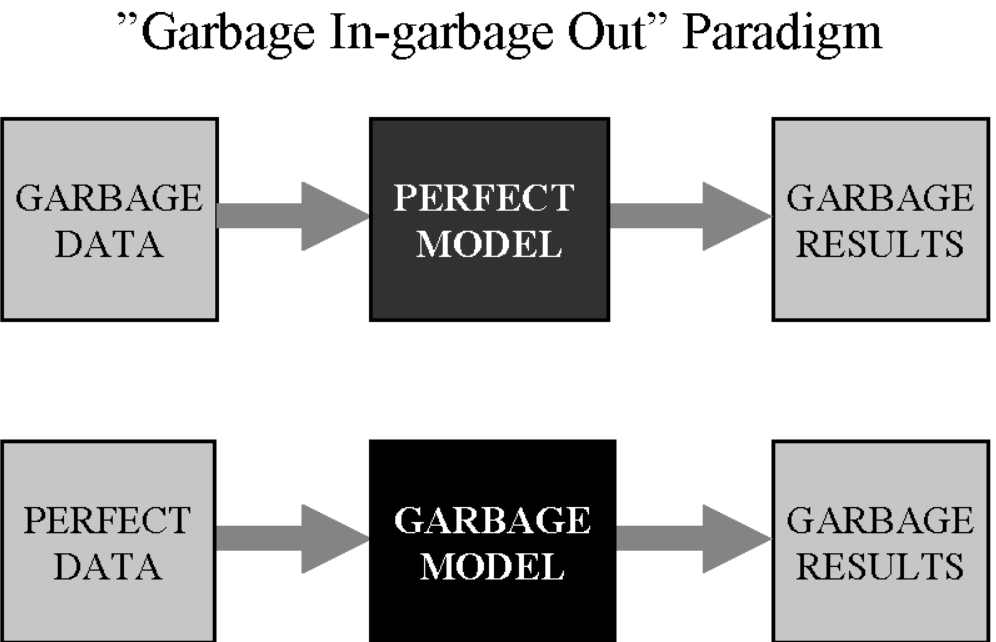
\includegraphics[height=7cm, width=12cm]{Fig/garb}
	%\end{figure}

%\end{frame}
%%%%%%%%%%%%%%%%%%%%%%%%%%
%% CONSIDERAÇÕES FINAIS
%%%%%%%%%%%%%%%%%%%%%%%%%%%%%%%%%%%%%%%%%%%%%%%%%%%%%%%%%%%%%%%%%%%%%%%%%%%%%%%%%%%%%%%%%%%%%%%%%%%%%%%%%%%%%%%%%
%\begin{frame}[t]{Considerações Finais}

    %\begin{variableblock}{Alternativa potencial}{bg=white,fg=black}{bg=black,fg=white}
	%\justifying
	%Os algorítimos de ML devem ser concebidos como uma \textcolor{blue}{alternativa %potencial} para solucionar problemas florestais mais complexos, para os quais os %métodos tradicionais não se mostraram satisfatórios. \\~\\
	%\end{variableblock}
	
	%\begin{variableblock}{Dados de qualidade}{bg=white,fg=black}{bg=black,fg=white}
	%\justifying
	%O limite do modelo em representar a realidade é, em boa parte, determinado pela %qualidade dos dados. \textcolor{blue}{Os modelos serão tão bons quanto os dados %utilizados para ensinar!} \\~\\
	%\end{variableblock}
	%\Springtree[3]
%\end{frame}

%%%%%%%%%%%%%%%%%%%%%%%%%%%%%%%%%%%%%%%%%%%%%%%%%%%%%%%%%%%%%%%%%%%%%%%%%%%%%%%%%%%%%%%%%%%%%%%%%%%%%%%%%%%%%%%%%%%%%%%%%%
%% PUBLICAÇÃO FUTURA
%%%%%%%%%%%%%%%%%%%%%%%%%%%%%%%%%%%%%%%%%%%%%%%%%%%%%%%%%%%%%%%%%%%%%%%%%%%%%%%%%%%%%%%%%%%%%%%%%%%%%%%%%%%%%%%%%%%%%%%%%%

%\begin{frame}[t]{}
	
	%\begin{figure}[h]
		%\centering
	    %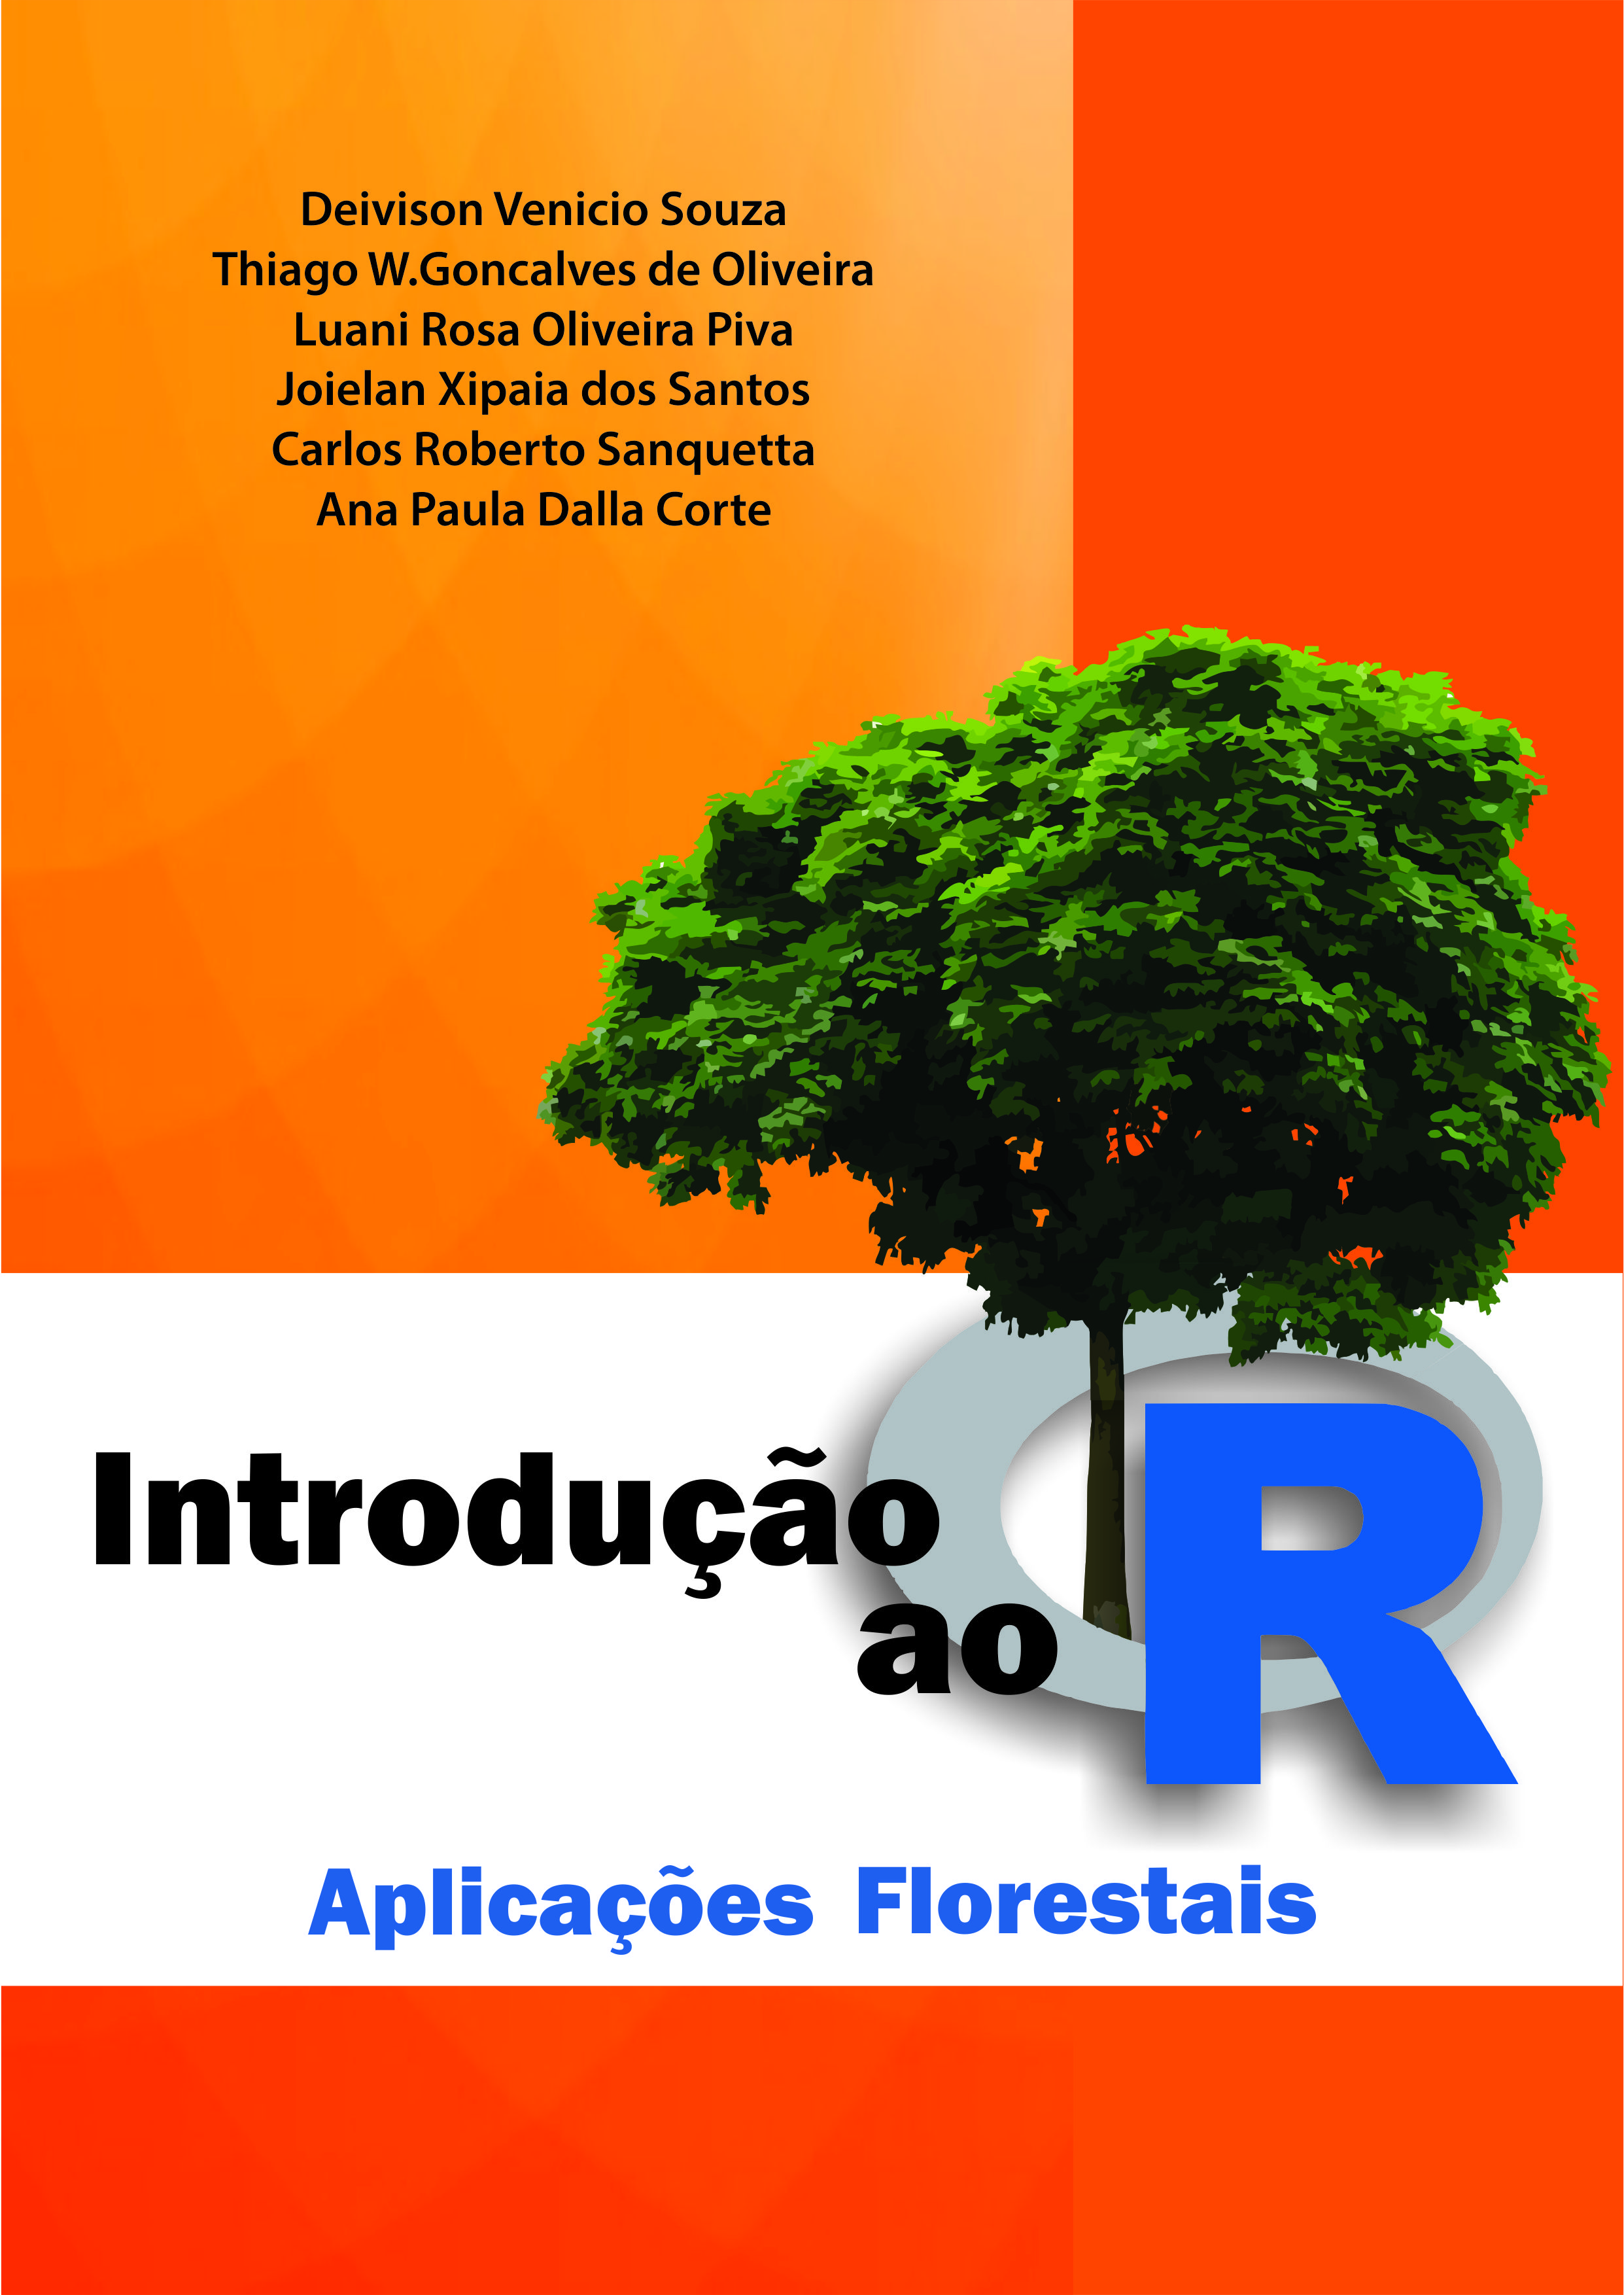
\includegraphics[width=6cm, height=8cm]{Fig/Livro.jpg}
	    %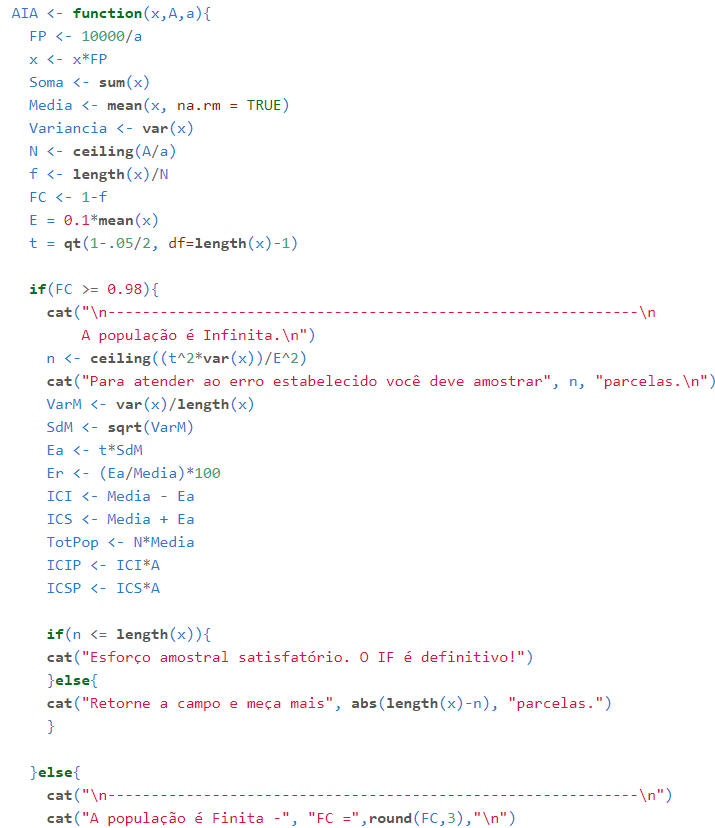
\includegraphics[width=6cm, height=8cm]{Fig/img8.png}
	%\end{figure}
	
%\end{frame}	

%%%%%%%%%%%%%%%%%%%%%%%%%%%%%%%%%%%%%%%%%%%%%%%%%%%%%%%%%%%%%%%%%%%%%%%%%%%%%%%%%%%%%%%%%%%%%%%%%%%%%%%%%%%%%%%%%%%%%%%%%%
%% BIBLIOGRAFIA
%%%%%%%%%%%%%%%%%%%%%%%%%%%%%%%%%%%%%%%%%%%%%%%%%%%%%%%%%%%%%%%%%%%%%%%%%%%%%%%%%%%%%%%%%%%%%%%%%%%%%%%%%%%%%%%%%%%%%%%%%%

\begin{frame}[t,allowframebreaks]{Bibliografia}
	\bibliography{refs}
\end{frame}

%%%%%%%%%%%%%%%%%%%%%%%%%%%%%%%%%%%%%%%%%%%%%%%%%%%%%%%%%%%%%%%%%%%%%%%%%%%%%%%%%%%%%%%%%%%%%%%%%%%%%%%%%%%%%%%%%%%%%%%%%%
%% AGRADECIMENTO
%%%%%%%%%%%%%%%%%%%%%%%%%%%%%%%%%%%%%%%%%%%%%%%%%%%%%%%%%%%%%%%%%%%%%%%%%%%%%%%%%%%%%%%%%%%%%%%%%%%%%%%%%%%%%%%%%%%%%%%%%%

\begin{frame}[c]{}
	
	\begin{center}
		{\Large \textbf{OBRIGADO!}} \\~\\
		Deivison Venicio Souza (UFPA) \\
		Email: deivisonvs@ufpa.br \\~\\
		\Springtree[5]
	\end{center}
	
\end{frame}

\end{document}

%%%%%%%%%%%%%%%%%%%%%%%%%%%%%%%%%%%%%%%%%%%%%%%%%%%%%%%%%%%%%%%%%%%%%%%%%%%%%%%%%%%%%%%%%%%%%%%%%%%%%%%%%%%%%%%%%%%%%%%%%%